\documentclass[usenames,dvipsnames,letterpaper,landscape,final]{slides}

\def\fileHome{.}
\def\icons{\fileHome/icons}

\input mySlideStyle2019-1.tex
\def\myfboxBlack#1{\fboxrule2pt\fbox{$\ds#1$}}
\newcommand\topSeparatorHeading[1]{\noPagetrue\begin{myslide}\headingline\vbox to5.5in{%
\vfil\begin{center}{{\large\myfboxBlack{\myfboxBlack{%
\text{\ \ \bf\Blue{\begin{tabular}{c}#1\end{tabular}\ \ }}}}}}%
\end{center}\vfil}\end{myslide}\noPagefalse}

\usepackage{multirow}
\usepackage{enumitem}
\usepackage[ruled,vlined]{algorithm2e}
%\usepackage{wallpaper}
		  \usepackage{mathtools}



\newcounter{outlineNumber}\setcounter{outlineNumber}{0}
\def\outno{\stepcounter{outlineNumber}\Blue{\theoutlineNumber. }}

\definecolor{boxColor}{rgb}{.4, .05, .2}

%------------------------------------------------------------------------------
\tikzset{cross/.style={cross out, draw=black, minimum size=2*(#1-\pgflinewidth), inner sep=0pt, outer sep=0pt},cross/.default={1pt}}

\renewcommand\floatpagefraction{0}
\renewcommand\textfraction{0}
\renewcommand\topfraction{1}
\renewcommand\bottomfraction{1}
\setcounter{topnumber}{10}
\setcounter{bottomnumber}{10}
\setcounter{totalnumber}{10}

\def\picWidth#1#2{\includegraphics[clip=true,keepaspectratio=true,width=#1]{#2}}
\def\picHeight#1#2{\includegraphics[clip=true,keepaspectratio=true,height=#1]{#2}}
\def\picWidthHeight#1#2#3{\includegraphics[clip=true,width=#1,height=#2]{#3}}

%\let\itemOld=\item
%\def\item{\parskip=0pt\itemsep=0pt\itemOld}

\let\dOrig=\d
\renewcommand{\d}{\partial}
\let\ReOrig=\Re
\renewcommand{\Re}{{\mathbb R}}

\def\grad{\nabla}
\let\divOrig=\div
\renewcommand\div{\nabla\cdot}

%\newcommand\0{\phantom{0}}

\def\dt{{\Delta t}}
\def\dx{{\Delta x}}
\def\dy{{\Delta y}}

\def\cA{{\mathcal{A}}}
\def\cD{{\mathcal{D}}}
\def\cF{{\mathcal{F}}}
\def\cL{{\mathcal{L}}}
\def\cO{{\mathcal{O}}}

\def\bv{{\bf v}}
\def\bE{{\bf E}}
\def\bx{{\bf x}}

\def\CFL{{\rm CFL}}

\def\Line(#1,#2)(#3,#4){\qbezier(#1,#2)(#1,#2)(#3,#4)}
\def\twoVec(#1,#2){\bigg(\begin{matrix}#1\\#2\end{matrix}\bigg)}


\def\d{\partial}
\def\grad{\nabla}
\def\div{\nabla\cdot}
\def\Div{\text{\rm div}}
\def\<{\langle}
\def\>{\rangle}

\let\vv=\v
%\def\G{\mathbf{G}}
\def\u{\mathbf{u}}
\def\U{\mathbf{U}}
\def\v{\mathbf{v}}
\def\V{\mathbf{V}}
\def\bpsi{\pmb{\psi}}
\def\bPsi{\pmb{\Psi}}
\def\bsigma{\pmb{\sigma}}
\def\bbV{{\mathbb{V}}}
\def\bbW{{\mathbb{W}}}

\def\cE{{\cal E}}
\def\cO{{\cal O}}
\def\cP{{\cal P}}
\def\cT{{\cal T}}

\def\D{\text{\rm D}}

\def\Po{\mathbb P}
\def\Re{\mathbb R}
\def\V{{\mathbb V}}
\def\W{{\mathbb W}}
\def\X{{\mathbb X}}

\def\cD{\mathcal{D}}
\def\cE{\mathcal{E}}
\def\cF{\mathcal{F}}
\def\cN{\mathcal{N}}
\def\cP{\mathcal{P}}
\def\cT{\mathcal{T}}

\def\RT{{\rm RT}}
\def\BR{{\rm BR}}
\def\St{{\rm S}}
\def\TH{{\rm TH}}
\def\J{{\text{\rm J}}}

\def\smallTwoVec(#1,#2){\Big(\begin{matrix}#1\\#2\end{matrix}\Big)}

\begin{document}

\begin{myslide}
\headingline
		  \vspace*{-30pt}{\bf\Large\begin{center}
					 Simulation of Multiphase Flow and Transport in Partially Melted Materials
		  \end{center}}

\vfill

\begin{center}{\obeylines
Chenyu Tian
\bigskip
		  {\it\OliveGreen{CSEM} 
		  \Blue{\it Oden Institute}}
\BurntOrange{The University of Texas at Austin}}
\end{center}

\vfill

		  \begin{center}
					 Todd Arbogast, Oden Institute \& Mathematics, University of Texas at Austin\\
Marc A. Hesse, Oden Institute \& Geosciences, University of Texas at Austin\\
		  \end{center}

		  \vspace*{10pt}

\end{myslide}
% ===========================================================
%\begin{myslideNoFooter}
%		  \heading{Darcy-Stokes system}
%\Blue{Darcy's law} for the fluid
%\begin{alignat*}3
%		  &\phi_f\v_r + \frac{k_0\phi^{2+2\Theta}}{\mu_f}\grad(p_f - \rho_f \mathbf{g}) &&= 0
%   &&\quad\OliveGreen{\text{(Darcy law)}}\\
%		  &\div(\phi_f\v_r + \v_s) &&= 0 
%   &&\quad\OliveGreen{\begin{aligned}&\text{(conservation/}\\&\ \text{compaction)}\end{aligned}}\\
%\intertext{\Blue{Stokes system} for a highly viscous, compressible matrix plus fluid}
%		  &\grad \bar{p} - \div\hat\bsigma(\v_s) &&= \bar{\rho}\mathbf{g}
%    &&\quad\OliveGreen{\text{(Stokes)}}\\
%&\mu_s\div \v_s - \phi_f\big(p_f - p_s) &&= 0
%    &&\quad\OliveGreen{\text{(compaction)}}
%\end{alignat*}
%
%\subhead{Assumption.} The divergence and gradient terms are well defined if
%\vspace*{-4pt}\begin{equation*}
%\myfbox{\phi\in L^\infty(\Omega)\text{ and }\phi^{\Theta-1/2}\grad\phi\in(L^\infty(\Omega))^d}
%\end{equation*}

%\subhead{Remarks.} Where $\phi=0$:
%\begin{blist}
%\item The scaled fluid pressure $\tilde q_f$ remains defined and bounded
%\item We do not lose the second equation
%\item Ignoring gradients, terms divided by $\phi$ are zero when $\phi=0$
%\end{blist}

%		  \subhead{Remarks.} The Darcy part will mathematically degenerate in regions where the 
%		  porosity is zero.

%\end{myslideNoFooter}

% Add motivation
\begin{myslideNoFooter}
          \heading{Motivation}
          \parbox{0.6\textwidth}{\raggedright
          \subhead{Partial Melting}
          \begin{nlist}
          \item Generates the oceanic and continental crust.
          \item Determines the large-scale chemical evolution of the Earth.
          \item Similar process may occur on other terrestrial planets.
          \end{nlist}
          }\parbox{0.4\textwidth}{\raggedright
          \begin{center}
               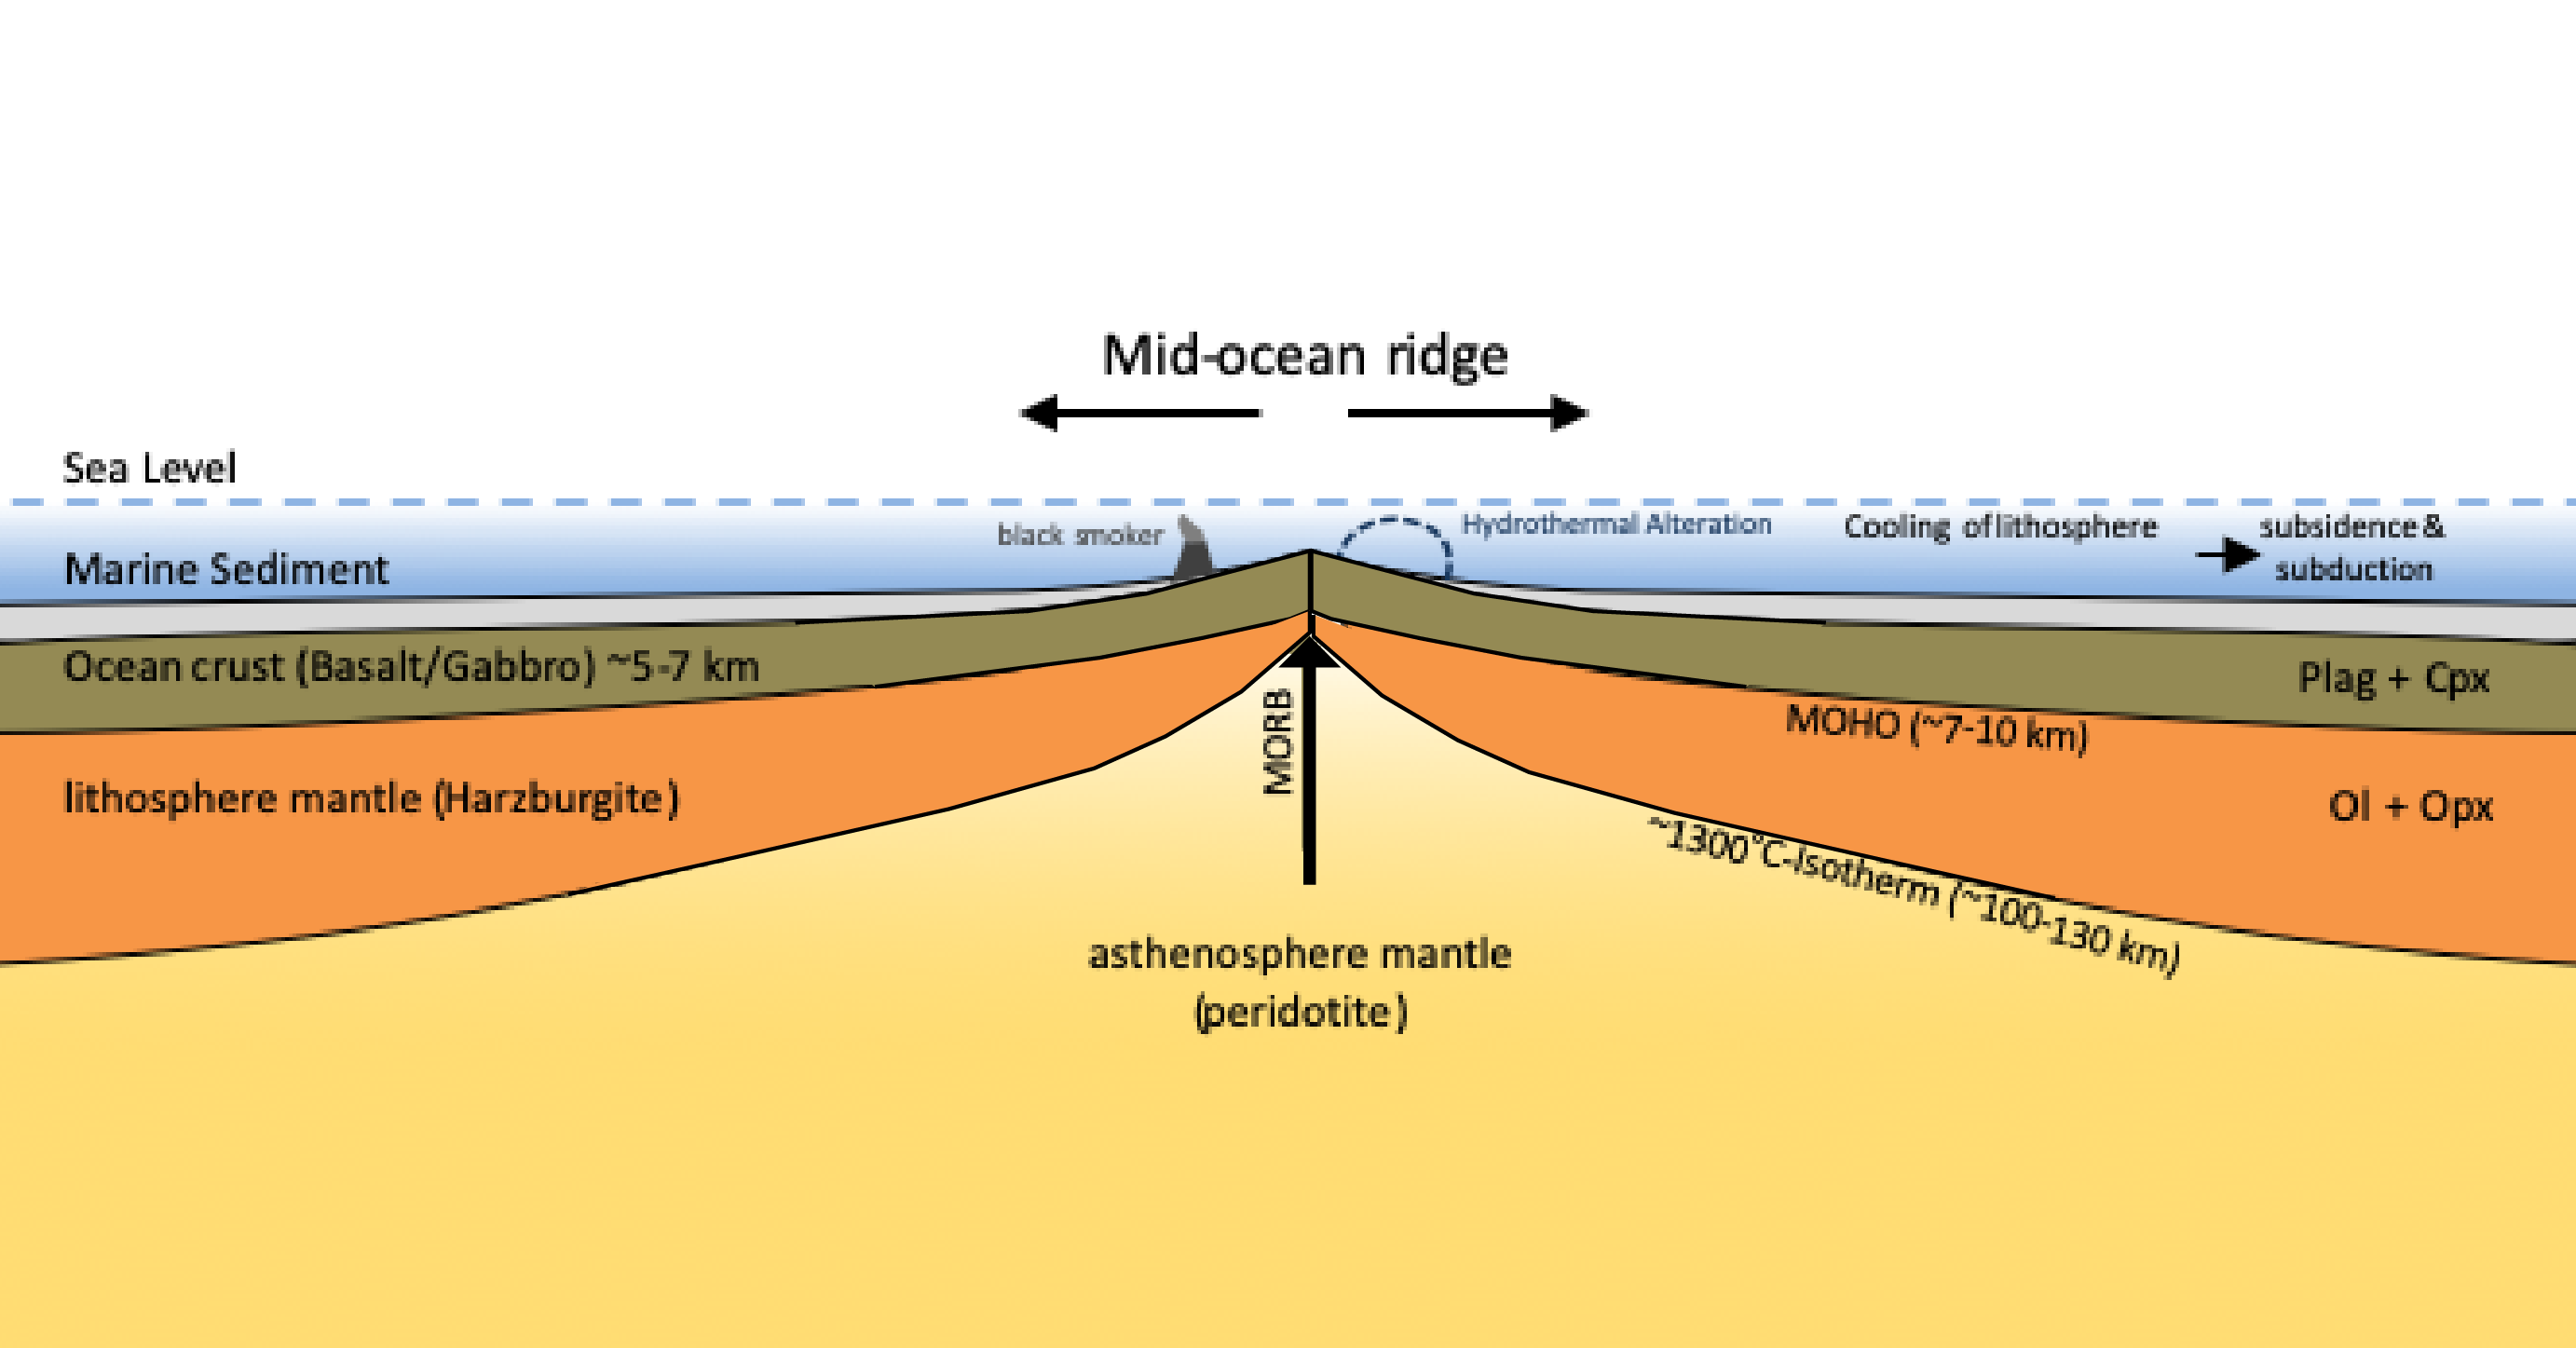
\includegraphics[width=9cm,height=7cm]{mid}
          \end{center} 
          (Mid-ocean ridge, Wikipedia)
          }
          
          \bigskip
          \subhead{Goals.}
          \begin{blist}
          \item Refine mathematical model governing the system.
          \item Develop a new code for simulation of partial melting process.
          \begin{blist}
          \item New mixed finite element space.
          \item Implement implicit WENO-AO method.
          \item Eutectic binary phase behavior.
          \end{blist}
          \item Perform numerical simulation help understanding of physics.
          \end{blist}
          
\end{myslideNoFooter}

\separatorHeading{\outno The Equations Governing Partially\\ Melting System}

\begin{myslideNoFooter}
\heading{Partially Melting System}
\parbox{\textwidth}{\parbox{0.53\textwidth}{\raggedright
\subheading{Elementary Representative Volume.}
\centering
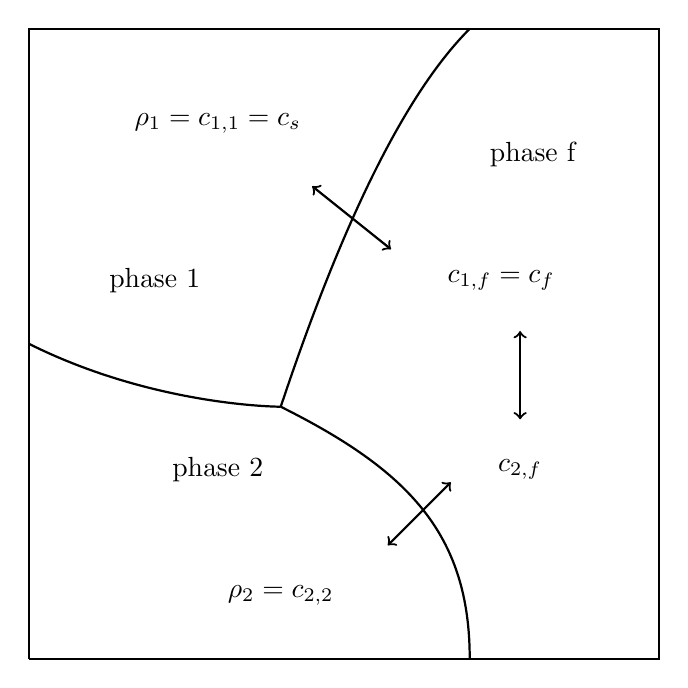
\begin{tikzpicture}[scale=0.4]
    \draw [thick] (0,0) -- (20,0) -- (20,20) -- (0,20) -- (0,0);
    \draw [thick] (0,10) .. controls (4,8) and (8,8) .. (8,8);
    \draw [thick] (8,8) .. controls (10,14) and (12,18) .. (14,20);
    \draw [thick] (8,8) .. controls (12,6) and (14,4) .. (14,0);
    
    \draw (8,2) node {$\rho_2=c_{2,2}$};
    \draw (6,17) node {$\rho_1=c_{1,1}=c_s$};
    \draw (15,12) node {$c_{1,f}=c_{f}$};
    \draw (15.6,6) node {$c_{2,f}$};

    \draw [thick, <->] (11.4,3.6) -- (13.4,5.6);
    \draw [thick, <->] (9,15) -- (11.5,13);
    \draw [thick, <->] (15.6,7.6) -- (15.6,10.4);
    
    \draw (4,12) node {phase 1};
    \draw (6,6) node {phase 2};
    \draw (16,16) node {phase f};
\end{tikzpicture}
}
\parbox{0.46\textwidth}{\raggedright
\subheading{Mixture theory for Mantle Dynamics}(McKenzie 1984)
Both fluid ($f$) and solid ($s$) phases
exist at each point of the domain $\Omega$.

Define the \Maroon{mixture variable} as:
\begin{equation*}
\begin{aligned}
\overline{\Psi} &= \phi \Psi_f + (1-\phi) \Psi_s = \Psi_s + \phi \Psi_r,\\
\Psi_r &= \Psi_f - \Psi_s. 
\end{aligned}
\end{equation*}}
}
\bigskip

\subhead{Governing equations}
\begin{nlist}
\item \Maroon{Darcy for fluid melt.} Fluid Melts between rock crystals, forming a porous medium.
\item \Maroon{Stokes for solid rock.} Highly viscous creep of the solid mantle.
\item \Maroon{Transport for thermodynamics.} Transport energy and mass. 
\item \Maroon{Phase behavior.} Approximated with binary eutectic phase behavior.
\end{nlist}

\end{myslideNoFooter}

\begin{myslideNoFooter}
\heading{Concentration of Components}
Let $c_{i,j}$ denote the concentration of component~$i$ in phase $j$. $M_{i,j}$ and $V_{i,j}$ are the mass and volume of component~$i\in\{1,2\}$ in phase~$j\in\{1,2,f\}$.

\subhead{Within Phase 1.}
\begin{equation*}
    c_s = c_{1,1} = \rho_1 = \frac{M_{1,1}}{V_1},\qquad c_{2,1} = 0 = M_{2,1},
\end{equation*}

\subhead{Within Phase 2.}
\begin{equation*}
	c_{1,2} = 0 = M_{1,2},\qquad c_{2,2} = \rho_2 = \frac{M_{2,2}}{V_2},
\end{equation*}

\subhead{Within Fluid Phase.}
\begin{equation*}
	c_f = c_{1,f} = \frac{M_{1,f}}{V_f},
	\qquad c_{2,f} = \frac{M_{2,f}}{V_f}.
\end{equation*}

\subhead{Phase Porosity}
\begin{equation*}
	\phi_f = \frac{V_f}{V},\qquad \phi_1 = \frac{V_1}{V},\qquad \phi_2 = \frac{V_2}{V},
\end{equation*}

\end{myslideNoFooter}
% ==================================================

\begin{myslideNoFooter}
\heading{Mixture Variables}
Considering only solid and fluid phases.
\begin{equation*}
\phi_s = \phi_1 + \phi_2 = 1 - \phi_f.
\end{equation*}
We now can define classic variables for mixture theory, considering $p_s=p_1=p_2$, $\v_s = \v_1 = \v_2$ in the solid phases and $p_f$, $\v_f$ in the fluid.
\bigskip

\subhead{Variables.}
\parbox{.5\textwidth}{
\begin{dlist}
\item[$\v_f, \v_s$] Phase velocity 
\item[$p_f, p_s$] Phase pressure 
\item[$\rho_f, \rho_s$] Phase density 
\item[$\mu_f, \mu_s$] Phase viscosity 
\item\strut
\item[$\rho_r=\rho_f-\rho_s$\,] Relative density 
\end{dlist}}\parbox{.5\textwidth}{
\begin{dlist}
\item[$\u$] Darcy velocity
\item[$\bar p$] Mixture pressure %$\phi p_f + (1-\phi)p_s$
\item[$\bar\rho$] Mixture density
\item[$\mathbf{g}$] Gravity vector 
\item\strut
\item[$\v_r=\v_f-\v_s$] Relative velocity 
\end{dlist}}



\end{myslideNoFooter}

% ===========================================================

\separatorHeading{Mechanics of Flow}

\begin{myslideNoFooter}
          \heading{Darcy system}
          \subhead{Darcy's Law}.
          \vspace*{-2pt}\begin{equation*}
\u = \phi_f \v_r = \phi_f (\v_f-\v_s)
 = -\frac{k_0 \phi_f^{2+2\Theta}}{\mu_f} (\grad p_f - \rho_f \mathbf{g})
\end{equation*}
The relative permeability $k(\phi)=\phi_f^{2+2\Theta}k_0$ for simplicity
          
\bigskip  
\subhead{Conservation of mass}
\vspace*{-6pt}\begin{equation*}
\frac{\d}{\d t}\bar\rho + \div\overline{\rho\v} = 0
\end{equation*}

\bigskip          

\Maroon{Boussinesq approximation}
For constant and equal densities for non-buoyancy terms
\begin{equation*}
\div\bar\v = \div(\phi_f \v_r + \v_s) = 0
\end{equation*}

\end{myslideNoFooter}

\begin{myslideNoFooter}
          \heading{Stokes system}
          \subhead{Viscous Stokes equation}. 
          
          Conservation of momentum for
the deviatoric stress of the mixture is
\begin{equation*}
\div\hat{\bsigma} = -\bar\rho\mathbf{g}
\end{equation*}
where
\begin{equation*}
    \hat{\boldsymbol\sigma}(\v_s)
    = 2\mu_s\phi_s\big(\cD\v_s - \tfrac{1}{3}\div\v_s\mathbf{I}\big)
\end{equation*}
The symmetric gradient is defined as:
\begin{equation*}
\cD\v_s=\frac12(\grad\v_s + \grad\v_s^T)
\end{equation*}

The equation for this mixture stress is therefore
\begin{equation*}       
\grad \bar p - \div\big(2\phi_s \mu_s\big(\cD \v_s
                           - \tfrac13\div \v_s\,\mathbf{I}\big)\big) = \bar\rho\mathbf{g}
\end{equation*}       

\subhead{Compaction}
\begin{equation*}
\phi_f(p_s - p_f) = -\mu_s \div \v_s,
\end{equation*}

\end{myslideNoFooter}

\begin{myslideNoFooter}
\heading{Reformation}
\subhead{Pressure Potentials.} Eliminate $p_s$ from system.
\begin{equation*}
	q_f = p_f - \rho_f g z\quad\text{and}\quad q_s = p_s - \rho_f g z,
\end{equation*}
\begin{equation*}
	p_f - p_s = q_f - q_s = \frac{1}{1-\phi_f}(q_f - q).
\end{equation*}
where $q = \bar{q}$. We can now rewrite the system with pressure potentials
\begin{equation*}
\begin{aligned}
	&\phi_f\v_r + \frac{k_0\phi_f^{2+2\Theta}}{\mu_f}\grad q_f &&= 0, &&&\Maroon{\text{(Darcy law)}}\\
	&\mu_s\div(\phi_f\v_r) + \frac{\phi_f}{1-\phi_f}(q_f-q) &&=0, &&&\Maroon{\text{(conservation}}\\
	&  && &&&\Maroon{\text{/compaction)}}\\
    &\grad q - \div\hat\bsigma(\v_s) &&= -(1-\phi_f)\rho_r\mathbf{g}, &&&\Maroon{\text{(Stokes)}}\\
	&\mu_s\div\v_s - \frac{\phi_f}{1-\phi_f}(q_f-q) &&=0  &&&\Maroon{\text{(compaction)}}.
	\end{aligned}
\end{equation*}
where
\begin{equation*}
\begin{aligned}
    \hat{\boldsymbol\sigma}(\v_s)
    &= 2\mu_s\phi_s\big(\cD\v_s - \tfrac{1}{3}\div\v_s\mathbf{I}\big) &&\Maroon{\text{(deviatoric stress of mixture)}}\\
   \cD\v_s&=\frac12(\grad\v_s + \grad\v_s^T) &&\Maroon{\text{(symmetric gradient)}}
    \end{aligned}
\end{equation*}

\end{myslideNoFooter}

% Tell Darcy and Stokes system separately

\begin{myslideNoFooter}
\heading{Scaled variables}
\subhead{Problem.} When no melt, $\phi_f = 0$, 
\begin{nlist}
\item Darcy system degenerates when $\phi_f$ vanishes, loss bound on $q_f$.
\item Lose the conservation equation.
\item The condition number grows as $\phi_f \rightarrow 0$
\end{nlist}
         \subhead{Scaled variables}\newline
          Define by Arbogast and Taicher [1]:
		  \begin{equation*}\label{eq:scaledVariables}
	\tilde\v_r = \phi_f^{-\Theta}\v_r
	\quad\text{and}\quad
	\tilde{q}_f = \phi_f^{1/2}q_f,
\end{equation*}
\subhead{The space $H_{\phi}(\text{div})$}\newline
$H_\phi(\Div;\Omega)$ is a Hilbert space with the inner-product\vspace*{-6pt}
\begin{equation*}
(\u,\v)_{H_\phi(\Div)} = (\u,\v) + \big(\phi^{-1/2}\div(\phi^{1+\Theta}\u),\phi^{-1/2}\div(\phi^{1+\Theta}\v)\big).
\end{equation*}\vspace*{-20pt}\newline
Moreover, $H(\Div;\Omega) = H_1(\Div;\Omega) \subset H_\phi(\Div;\Omega)$.

	
\end{myslideNoFooter}

\begin{myslideNoFooter}
		  \heading{Scaled Formation}
		  \subhead{New formation with scaled variables}
        \begin{alignat*}2
    &\tilde\v_r
        + \frac{k_0\phi_f^{1+\Theta}}{\mu_f}\grad(\phi_f^{-1/2}\tilde q_f)
        &&= 0,\\
    &\mu_s\phi^{-1/2}\div(\phi_f^{1+\Theta}\tilde\v_r)
        + \frac{1}{1-\phi_f}(\tilde{q}_f - \phi_f^{1/2}q) &&=0,\\
    &\grad q - \div\hat\bsigma(\v_s) &&= -(1-\phi_f)\rho_r \mathbf{g},\\
    &\mu_s\div\v_s
        - \frac{\phi_f^{1/2}}{1-\phi_f}(\tilde{q}_f - \phi_f^{1/2}q) &&=0.
		  \end{alignat*}

\Maroon{Boundary conditions}
\begin{equation*}
    \phi_f\v_r\cdot\nu = \phi_f^{1+\Theta}\tilde\v_r\cdot\nu = g_{r}
    \quad\text{and}\quad \v_s = \mathbf{g}_{s} \quad\text{on }\d\Omega,
\end{equation*}

\Maroon{Compatibility}
\begin{equation*}
	\int_{\d\Omega}(g_r + \mathbf{g}_s \cdot \nu)\,ds = 0.
\end{equation*}

\end{myslideNoFooter}
% ===========================================================

\separatorHeading{Transport of Mass and Energy}

\begin{myslideNoFooter}
		  \heading{Mass transport system}
		  \subhead{Mass Transport Equation}
		  \begin{equation*}
    \bar{c}_t + \div (\overline{c\v} - \phi_f D \grad c_f)=0,
\end{equation*}
where bulk transport variable is defined
\begin{equation*}
	\bar{c} = \phi_f c_f + \phi_1 c_s
	= \frac{V_f}{V}\frac{M_{1,f}}{V_f} + \frac{V_1}{V}\frac{M_{1,1}}{V_1}
	= \frac{M_{1,f} + M_{1,1}}{V}
	= \frac{M_1}{V}
\end{equation*}

\bigskip
\Maroon{Standard solving approach proposed by Katz.}
\begin{equation*}
\begin{aligned}
	&(\phi_f c_f)_t + \div (\phi_f c_f \v_f - \phi_f D \grad c_f)
	    &&= \Gamma,\\
	&(\phi_1 c_s)_t + \div (\phi_1 c_s \v_s) &&= -\Gamma.
\end{aligned}
\end{equation*}

\bigskip
\subhead{Note.}\begin{blist}
\item Set $\Gamma = 0$.
\item Perform flash calculation later to account for the melting term.
\end{blist}

\end{myslideNoFooter}
% ===========================================================
\begin{myslideNoFooter}
\heading{Partition Function}
A different approach to solve the mass transport equation 
without \Maroon{splitting} is proposed.

\subhead{Definition}
\begin{equation*}
	\phi_f c_f = \kappa(E,\bar{c})\,\bar{c},\qquad
    \kappa \coloneqq \frac{\phi_f c_f}{\bar{c}}, \qquad
    \kappa \in [0,1]
\end{equation*}

A simplified version of transport equation with partition function is 
therefore proposed.
\begin{equation*}
	\bar{c}_t + \div (\v_e \bar{c} - \kappa D \grad \bar{c}) = 0,
\end{equation*}
\Maroon{Effective Velocity}
\begin{equation*}
	 \v_e = \v_e^* - D (\grad \kappa - \kappa \grad \ln\phi_f)
	 = \kappa\v_r + \v_s - D(\grad\kappa - \kappa\grad \ln\phi_f),
\end{equation*}

\end{myslideNoFooter}


% ===========================================================

\begin{myslideNoFooter}
		  \heading{Energy transport system}
		  \subhead{Energy Transport}
		  \begin{equation*}
	E_t + \div(\overline{\rho e\v} - \bar{K} \grad T) = 0,
\end{equation*}
where transport variable is defined
		  \begin{equation*}
    E = \overline{\rho e}
    = \phi_f\rho_f e_f + \phi_1\rho_1 e_1 + \phi_2\rho_2 e_2.
\end{equation*}

\subhead{Define partition function}
		  \begin{equation*}
	\phi_{f}\rho_{f}e_{f} = \lambda(E,\bar{c})\,E,
	\qquad\lambda \coloneqq \frac{\phi_f\rho_{f}e_f}{E},
	\qquad \lambda \in [0,1]
\end{equation*}
The resulting simplified energy transport function is therefore
\begin{equation*}
E_t + \div(\v_e^{E} E - \bar{K}\grad T) = 0,
\end{equation*}
\Maroon{Effective velocity}
		  \begin{equation*}
\v_e^{E} = \lambda\v_f + (1-\lambda)\v_s = \lambda\v_r + \v_s.
\end{equation*}

\end{myslideNoFooter}

% ===========================================================

\begin{myslideNoFooter}
\heading{Phase Behavior}
The flash calculation takes $\bar c$ and $E$ and gives $\phi_f$ and $T$, as well as $c_f$ and $\phi_1$.
A phase package is thus required.

\bigskip
\subhead{Binary Eutectic}
\begin{center}
    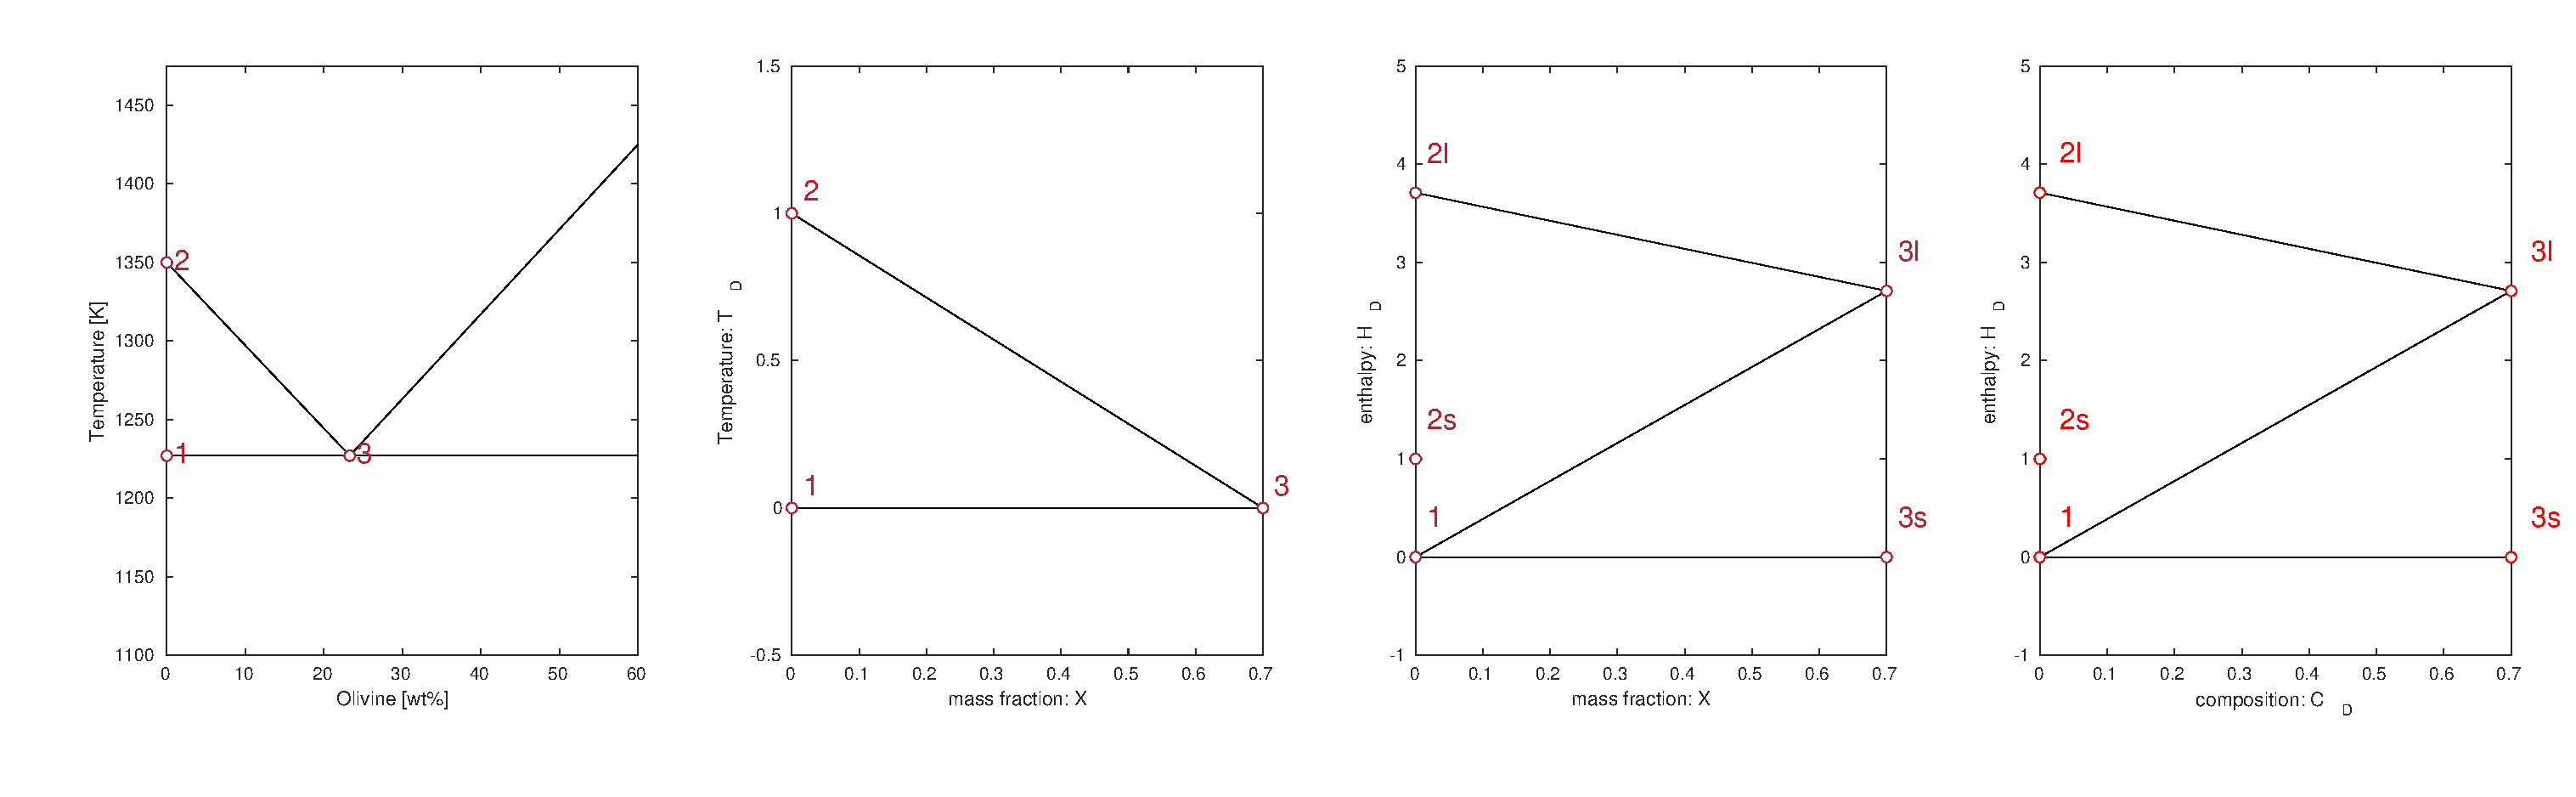
\includegraphics[height=8cm,width=20cm]{phase.eps}
\end{center}

\Maroon{Olivine} and \Maroon{pyroxene} are two usual immiscible cryctals in mantle melting process.


\end{myslideNoFooter}

% ===========================================================

\separatorHeading{\outno Computational Method}

\begin{myslideNoFooter}
\heading{Spatial and Time Discretization}
\bigskip
\begin{nlist}
\item \Blue{Conforming quadrilaterals.} Should be strictly convex and not degenerate into a triangle, line or point. Maintaining logical order when adjusting grid coordinates.
\item \Blue{Mixed finite element method.} Second order accuracy for smooth mechanical flow.
\item \Blue{Weighted essentially non-oscillatory method (WENO).} Shock capturing scheme for convection diffusion equation. Third order accuracy for velocities.
\item \Blue{Flash calculation.} An explicit, direct parametrization of the phase diagram.
\end{nlist}

\begin{center}
    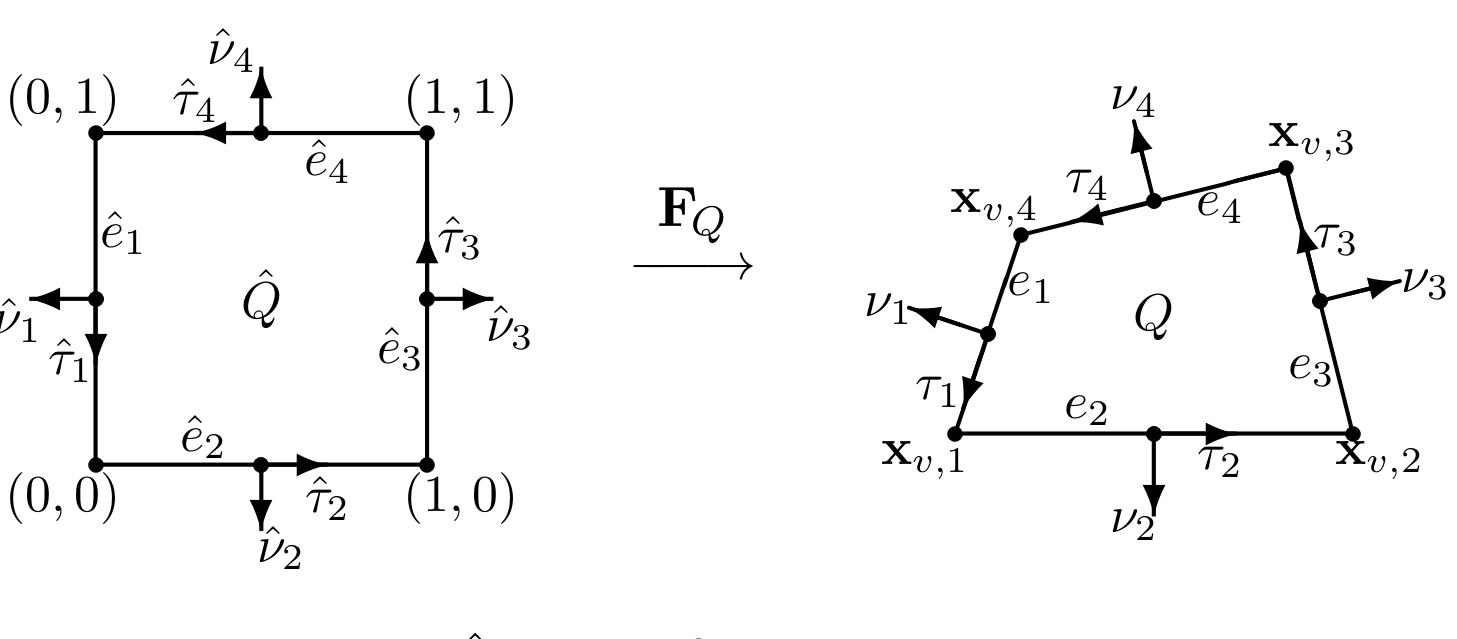
\includegraphics[width=14cm,height=6cm]{mesh.png}
\end{center}

\end{myslideNoFooter}

% ============================================================

\separatorHeading{A Mixed Finite Element Method \\ for flow}

\begin{myslideNoFooter}
\heading{A Scaled Weak Formulation}
\vspace*{-8pt}\begin{align*}
H_{\phi,0}(\Div;\Omega) &=\big\{\v\in(L^2(\Omega))^d :\\
&\qquad\phi^{-1/2}\div(\phi^{1+\Theta}\v)\in L^2(\Omega),\ \phi^{1/2+\Theta}\v\cdot\nu=0\text{ on }\d\Omega\big\}
\end{align*}   
               
\subhead{Scaled weak formulation.}
               
Find $\tilde\v_r\in H_{\phi,0}(\Div)$, $\tilde q_f\in L^2$, $\v_s \in(H_0^1)^d$, and $q\in L^2/\Re$ such that
\begin{alignat*}3
&\Big ( \frac{\mu_f}{k_0} \tilde{\v}_r, \bpsi_r \Big )
            - \big(\tilde q_f, \phi_f^{-1/2}\div (\phi_f^{1+\Theta}\bpsi_r)\big)
 &= 0\ &&&\forall\,\bpsi_r \in H_{\phi_f,0}(\Div)\\
&\big(\phi_f^{-1/2}\div(\phi_f^{1+\Theta}\tilde{\v}_r),w_f\big)
               + \Big(\frac1{\mu_s(1-\phi_f)}(\tilde q_f-\phi_f^{1/2}q),w_f\Big) &= 0\ &&&\forall w_f \in L^2\\
&\!-\!(q,\div \bpsi_s) + (\hat\bsigma(\v_s),\grad\bpsi_s) &\llap{$= (\mathbf{G},\bpsi_s)$}\ &
  &&\forall\,\bpsi_s \in(H_0^1)^d\\
&(\div \v_s,w) - \Big(\frac{\phi_f^{1/2}}{\mu_s(1-\phi_f)}(\tilde q_f - \phi_f^{1/2}q),w\Big)
  &= 0\ &&&\forall w\in L^2/\Re
\end{alignat*} 

\end{myslideNoFooter}

\begin{myslideNoFooter}
\heading{Mixed Finite Elements}
For a polygonal domain $\Omega \subset \Re^d \quad d = \{2,3\}$. Assume $d=2$ for now.

\subhead{For Darcy.} $\V_{\D} \times \W_{\D} \subset H_0(\Div;\Omega)\times L^2(\Omega)$.

\parbox{.7\textwidth}{\raggedright
\bigskip
Lowest order reduced $H$(div)-approximation AC space.
\begin{equation*}
\begin{aligned}
    \bbV_{D,h}(Q) &= \bbV_1^0(Q) = \mathbb{P}^2_1\oplus\textrm{curl}\,\mathbb{S}_1(Q)\\
    \bbW_{D,h}(Q) &= \bbW_1^0(Q) = \mathbb{P}_0,
   \end{aligned} 
\end{equation*}
\Maroon{Accuracy} $\cO(h^2)$ for $\tilde{\v}_r$ and $\cO(h)$ for $\tilde{q}_f$.

\Maroon{DOF} $8+1 = 9$.
}\parbox{0.3\textwidth}{
\centerline{\setlength\unitlength{4.5pt}
\begin{picture}(30,30)(-15,-15)
\thicklines
\put(-10,-10){\line(1,0){20}}\put(-10,-10){\line(0,1){20}}
\put(10,10){\line(-1,0){20}}\put(10,10){\line(0,-1){20}}
\put(0,0){\PineGreen{\circle*{2}}}
\put(-10,2){\makebox(0,0){\Maroon{$\times$}}}
\put(-10,-2){\makebox(0,0){\Maroon{$\times$}}}
\put(-6,-2){\vector(-1,0){9}}\put(-6,2){\vector(-1,0){9}}
\put(10,2){\makebox(0,0){\Maroon{$\times$}}}
\put(10,-2){\makebox(0,0){\Maroon{$\times$}}}
\put(6,-2){\vector(1,0){9}}\put(6,2){\vector(1,0){9}}
\put(2,-10){\makebox(0,0){\Maroon{$\times$}}}
\put(-2,-10){\makebox(0,0){\Maroon{$\times$}}}
\put(-2,-6){\vector(0,-1){9}}\put(2,-6){\vector(0,-1){9}}
\put(2,10){\makebox(0,0){\Maroon{$\times$}}}
\put(-2,10){\makebox(0,0){\Maroon{$\times$}}}
\put(-2,6){\vector(0,1){9}}\put(2,6){\vector(0,1){9}}
\end{picture}}
}
\bigskip

\subhead{For Stokes.} $\V_{\St} \times \W_{\St} \subset (H_0^1(\Omega))^2\times L^2(\Omega)$

\parbox{.7\textwidth}{\raggedright
\bigskip
Modified Bernardi-Raugel element.
\begin{equation*}
\begin{aligned}
    \bbV_{S,h}(Q) &= \mathbb{DS}_1^2(Q)\oplus \text{span}\{\mathbf{b}_1, \mathbf{b}_2,\mathbf{b}_3, \mathbf{b}_4\}\\
    \bbW_{D,h}(Q) &= \bbW_1^0(Q) = \mathbb{P}_0,
    \end{aligned}
\end{equation*}
\Maroon{Accuracy} $\cO(h^2)$ for $\v_s$ and $\cO(h)$ for $q_h$

\Maroon{DOF} $12 + 1 = 13$
}\parbox{0.3\textwidth}{
\centerline{\setlength\unitlength{4.5pt}
\begin{picture}(30,30)(-15,-15)
\thicklines
\put(-10,-10){\line(1,0){20}}\put(-10,-10){\line(0,1){20}}
\put(10,10){\line(-1,0){20}}\put(10,10){\line(0,-1){20}}
\put(0,0){\PineGreen{\circle*{2}}}
\put(-10,0){\makebox(0,0){\Maroon{$\times$}}}\put(-6,0){\vector(-1,0){9}}
\put(10,0){\makebox(0,0){\Maroon{$\times$}}}\put(6,0){\vector(1,0){9}}
\put(0,-10){\makebox(0,0){\Maroon{$\times$}}}\put(0,-6){\vector(0,-1){9}}
\put(0,10){\makebox(0,0){\Maroon{$\times$}}}\put(0,6){\vector(0,1){9}}
\put(-10,-10){\makebox(0,0){\Maroon{$\otimes$}}}
\put(-10,10){\makebox(0,0){\Maroon{$\otimes$}}}
\put(10,-10){\makebox(0,0){\Maroon{$\otimes$}}}
\put(10,10){\makebox(0,0){\Maroon{$\otimes$}}}
\end{picture}}
}

\end{myslideNoFooter}

% =================================================

\begin{myslideNoFooter}
\heading{A Scaled Mixed Finite Element Method}
\subhead{Scaled mixed finite element method}
		  Find $\tilde\v_{r,h}\in\bbV_{D,h} + \boldsymbol{g}_r$, $\tilde{q}_{f,h}\in\bbW_{D,h}$, $\v_{s,h}\in\bbV_{S,h} + \boldsymbol{g}_s$, and $q_h\in\bbW_{S,h}$ such that
\begin{alignat*}2
    &\Big(\frac{\mu_f}{k_0}\tilde\v_{r,h},\bpsi_r\Big)
        - \big(\tilde{q}_{f,h},
            \phi_f^{-1/2}\div(\phi_f^{1+\Theta}\bpsi_r)\big) &&= 0,\\
    &\big(\phi_f^{-1/2}\div(\phi_f^{1+\Theta}\tilde\v_{r,h}),\omega_f\big)
        + \Big(\frac{1}{\mu_s(1-\phi_f)}(\tilde{q}_{f,h}
            - \phi_f^{1/2}q_h),\omega_f\Big) &&= 0,\\
    &(q_h,\div\bpsi_s) - \big(\bsigma(\v_{s,h}),\grad\bpsi_s\big) - ((1-\phi_f)\rho_r \mathbf{g},\psi_s)
        &&= 0,\\
    &(\div\v_{s,h},\omega)
        - \Big(\frac{\phi_f^{1/2}}{\mu_s(1-\phi_f)}
            (\tilde{q}_{f,h} - \phi_f^{1/2}q_h),\omega\Big) &&= 0,
\end{alignat*}

\bigskip
\subhead{Lemma.} There exists a unique solution to the discrete equations.

\subhead{Problems.}
\begin{blist}
\item $\phi_f^{-1/2}$ causes problem when $\phi_f \rightarrow 0$.
\item It is not locally conservative.
\end{blist}

\end{myslideNoFooter}

% =================================================

\begin{myslideNoFooter}
\heading{A Local Mass Conservation Modification}

\subhead{Locally averaged $\phi$}
On each mesh element $Q$, the average of $\phi_f$ is $\phi_{f,Q}$, then define
$\hat{\phi}_f\big|_Q = \phi_{f,Q}$ a constant. Using divergence theorem,
\begin{equation*}
\begin{aligned}
    \int_Q\hat\phi_f^{-1/2}\div(\phi_f^{1+\Theta}\bpsi_{r,h})\,\omega_f\,dx
&= \int_{\d Q}\phi_{f,Q}^{-1/2}\phi_f^{1+\Theta}\bpsi_{r,h}\cdot\nu\,\omega_f\,ds\\
\nonumber
&\quad-\int_Q\phi_{f,Q}^{-1/2}\phi_f^{1+\Theta}\bpsi_{r,h}\cdot\grad\omega_f\,dx.
\end{aligned}
\end{equation*}
The second integral will vanish when $\omega_f$ is constant on $Q$. We avoid problem of $\phi_f^{-1/2}$ when $\phi_f \rightarrow 0$.

\end{myslideNoFooter}
% ===================================================================

\begin{myslideNoFooter}
		  \heading{A Locally conservative method}
		  \subhead{Mixed finite element problem set up}
		  Find $\tilde\v_{r,h}\in\bbV_{D,h} + \hat{\boldsymbol{g}}_r$, $\tilde{q}_{f,h}\in\bbW_{D,h}$, $\v_{s,h}\in\bbV_{S,h} + \hat{\boldsymbol{g}}_s$, and $q_h\in\bbW_{S,h}$ such that
\begin{alignat*}2
    &\Big(\frac{\mu_f}{k_0}\tilde\v_{r,h},\bpsi_r\Big)
        - \big(\tilde{q}_{f,h},
            \hat\phi_f^{-1/2}\div(\phi_f^{1+\Theta}\bpsi_r)\big) &&= 0,\\
    &\big(\hat\phi_f^{-1/2}\div(\phi_f^{1+\Theta}\tilde\v_{r,h}),\omega_f\big)
        + \Big(\frac{1}{\mu_s(1-\phi_f)}(\tilde{q}_{f,h}
            - \phi_f^{1/2}q_h),\omega_f\Big) &&= 0,\\
    &(q_h,\div\bpsi_s) - \big(\hat\bsigma(\v_{s,h}),\grad\bpsi_s\big) - ((1-\phi_f)\rho_r \mathbf{g},\psi_s)
        &&= 0,\\
    &(\div\v_{s,h},\omega)
        - \Big(\frac{\hat\phi_f^{1/2}}{\mu_s(1-\phi_f)}
            (\tilde{q}_{f,h} - \phi_f^{1/2}q_h),\omega\Big) &&= 0,
\end{alignat*}
for all test functions $\bpsi_r\in\bbV_{D,h}$, $\omega_f\in\bbW_{D,h}$, $\bpsi_s\in\bbV_{S,h}$, and $\omega\in\bbW_{S,h}$.

\bigskip
\subhead{Retrieve local mass conservation} With $\omega_f = \phi_{f,Q}^{-1/2}\omega_Q \in\bbW_{D,h}$ and $\omega=\omega_Q\in\bbW_{S,h}$. We define $\omega_Q$ being 1, the sum of conservation/compaction and conservation equations results in
\begin{equation*}
    \int_Q\div(\phi_f^{1+\Theta}\tilde\v_r)\,dx + \int_Q\div\v_s\,dx = 0,
\end{equation*}

\end{myslideNoFooter}

\begin{myslideNoFooter}
\heading{Recovery of the unscaled Darcy variables}
The unscaled \Maroon{Darcy potential} is calculated as $q_f = \phi_f^{-1/2}\tilde{q}$. Assume that $q_{f,h} \in \bbW_{D,h}$, on $Q$ we define
\begin{equation*}
    q_{f,h}\big|_Q = \begin{cases}
    \phi_{f,Q}^{-1/2} \tilde q_{f,h}\big|_Q&\text{if }\phi_{f,Q}\ne0,\\
    0&\text{if }\phi_{f,Q}=0,
    \end{cases}
\end{equation*}

\subhead{Relative Darcy velocity} Given by $\v_r = \phi_f^\Theta\tilde\v_r$, and define the normal trace of $\v_{r,h} \in \bbV_{D,h}$ on each edge $e\subset\d Q$,
\begin{equation*}
    \int_{e}\phi_f^{1+\Theta}\tilde\v_{r,h}\cdot\nu\,ds
    = \int_{e}\phi_f\v_{r,h}\cdot\nu\,ds.
\end{equation*}
Using a weighted $L^2$ projection on the edge $e$, denoted as $P_1^{\phi_f}:L^2(e)\to\mathbb{P}_1(e)$ and defined by the requirement that for $f\in L^2(e)$, $P_1^{\phi_f}f\in\mathbb{P}_1(e)$ and
\begin{equation*}
    \int_e\phi_f(f-P_1^{\phi_f}f)\,\ell\,ds = 0
    \quad\forall\ell\in\mathbb{P}_1(e).
\end{equation*}
Then
\begin{equation*}
    \v_{r,h}\cdot\nu = P_1^{\phi_f}(\phi_f^\Theta \tilde\v_r\cdot\nu),
\end{equation*}

\end{myslideNoFooter}



% ==============================================================

\begin{myslideNoFooter}
\heading{Direct Serendipity Space}
\subhead{Auxiliary functions} In construction of the direct serendipity space, we start by defining auxiliary functions.
\begin{equation*}
       \lambda_i(\mathbf{x}) = -(\mathbf{x} - \mathbf{x}_{vi})\cdot\nu_i,\quad i=1,2,3,4,
\end{equation*}
Then define
\begin{equation*}
        R_{13}(\mathbf{x}) = \frac{\lambda_1 - \lambda_3}{\lambda_1 + \lambda_3},\quad
        R_{24}(\mathbf{x}) = \frac{\lambda_2 - \lambda_4}{\lambda_2 + \lambda_4},
\end{equation*}
and 
\begin{equation*}
  \begin{aligned}
 R_1(\mathbf{x}) &= \tfrac{1}{2}(1-R_{13}),\quad
        R_3(\mathbf{x}) = \tfrac{1}{2}(1+R_{13}),\\
 R_2(\mathbf{x}) &= \tfrac{1}{2}(1-R_{24}),\quad
        R_4(\mathbf{x}) = \tfrac{1}{2}(1+R_{24}).
 \end{aligned}
\end{equation*}
Function $R_i$ is 1 on corresponding edge $e_i$, 0 on the 
opposite edge, and arbitrary on two neighbours.
\begin{equation*}
    \mathbb{S}_1(Q) = \text{span}\big\{
        \lambda_2\lambda_4 R_{13},\ \lambda_1\lambda_3 R_{24}\big\},
\end{equation*}
    
\subhead{Resulted $\mathbb{DS}_1(Q)$ space}
\begin{equation*}
\mathbb{DS}_1(Q) = \mathbb{P}_1\oplus\mathbb{S}_1(Q),
\end{equation*}
Defined on the given quadrilateral $Q$.

\end{myslideNoFooter}
% ===================================================================

\begin{myslideNoFooter}
\heading{A Modified Bernardi-Raugel Element}
The modified Bernardi-Raugel finite element is
therefore defined as following:
\begin{equation*}
    \begin{aligned}
    \mathbb{V}_{S,h}(Q)&= \mathbb{DS}_1^2(Q)\oplus \text{span}\{\mathbf{b}_1, \mathbf{b}_2,\mathbf{b}_3, \mathbf{b}_4\}\\
    \mathbb{W}_{D,h}(Q) &= \mathbb{W}_1^0(Q) = \mathbb{P}_0,
\end{aligned}
\end{equation*}

\bigskip
\subhead{Supplemental functions} 

Four supplemental functions are defined modulo 4 by
\begin{equation*} 
     \mathbf{b}_i(\mathbf{x}) = \frac{\varphi_{i}(\mathbf{x})}{\varphi_{i}(\mathbf{x}_{i})} \nu_{i},\quad
     \mathbf{x}_i = \tfrac12(\mathbf{x}_{v,i-1}+\mathbf{x}_{v,i}),\quad
     \varphi_{i} = \lambda_{i+1}\lambda_{i+3}R_i,
\end{equation*}
We remark that the scalar function $\varphi_i$ lie in second order
serendipity space $\mathbb{DS}_2(Q)$.
\end{myslideNoFooter}

% =============================================================

\begin{myslideNoFooter}
\heading{Quadrilateral Mesh}

\begin{center}
    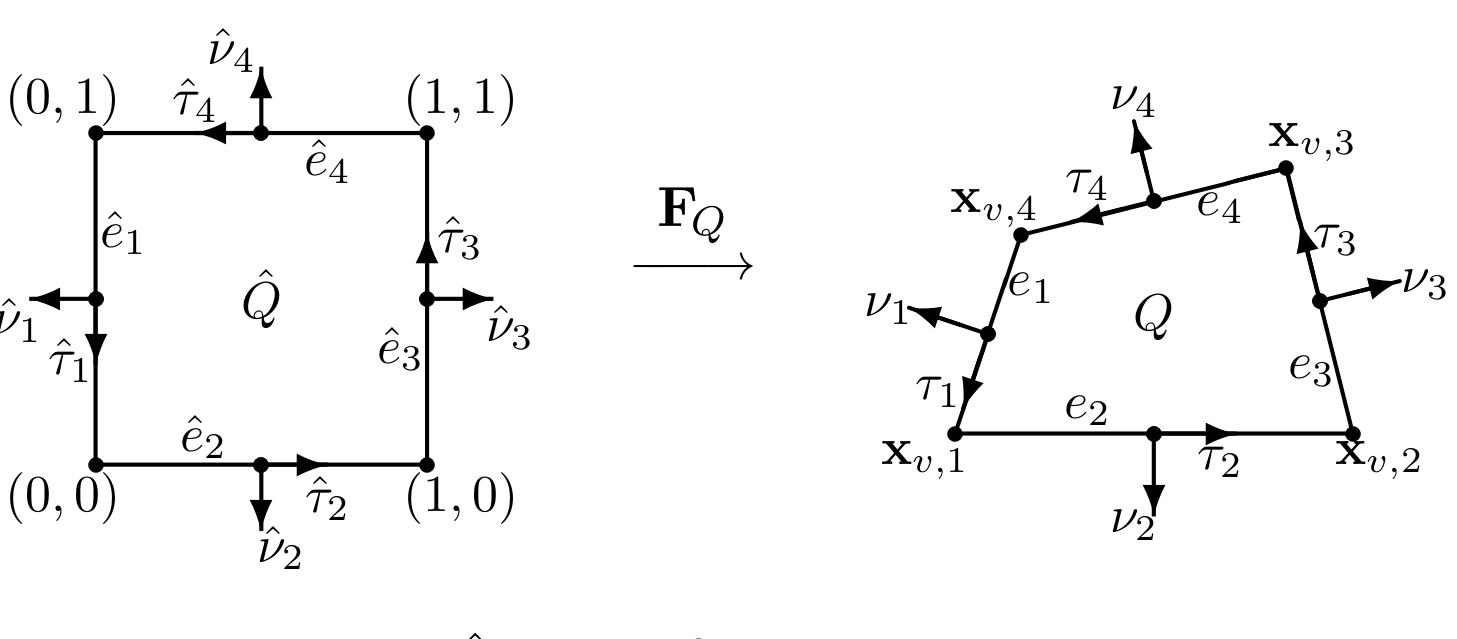
\includegraphics[width=14cm,height=6cm]{mesh.png}
\end{center}

\parbox{0.5\textwidth}{\raggedright
\subhead{Notations.}
\begin{blist}
\item $\nu_i$ Unit outer normal.
\item $\tau_i$ Unit tangent vector.
\item $e_i$ Edge middle point.
\item $\mathbf{x}_i$ Vertex points.
\end{blist}
}\parbox{0.5\textwidth}{\raggedright
\subhead{Advantages}
\begin{blist}
\item Fit complex geometry.
\item Require less element than triangular mesh.
\end{blist}
}

\subhead{Note.} 
\begin{nlist}
\item When \Maroon{$d=2$}, the convergence of the linear
serendipity finite element space does not degenerate on quadrilateral mesh.
\item Direct serendipity space defined directly on quadrilateral mesh without mapping from reference rectangular.
\end{nlist}

\end{myslideNoFooter}

% ===========================================================

\separatorHeading{WENO-AO Method for Transport}

\begin{myslideNoFooter}
		  \heading{Transport problem}
		  \subhead{Transport system equation}
		  \begin{equation*}
	U_t + \Div[ F(U) - A(U)\Grad U ] = 0,
\end{equation*}
where the transport variable is defined $U=(\bar c,E)$ row-wise. 

\bigskip
\subhead{Flux and diffusion coefficient matrices}
\begin{equation*}
F(U) = F\twoVec(\bar c,E) = \twoVec({\v_e^T\,\bar c},{(\v_e^E)^T E})
\quad\text{and}\quad
A(U) = \left[\begin{matrix}
\kappa D&0\\
\frac{\d T}{\d\bar c}&\frac{\d T}{\d E}
\end{matrix}\right],
\end{equation*}
	
In terms of the average of $U$ over the element $Q$,
\begin{equation*}
    U_Q(t) = \twoVec({\bar{c}_Q(t)} , {E_Q(t)}),
    \quad
    \bar{c}_Q(t) = \frac{1}{|Q|}\int_Q \bar c(x,t)\,dx,
\end{equation*}
and
\begin{equation*}
    E_Q(t) = \frac{1}{|Q|}\int_Q E(x,t)\,dx,
\end{equation*}

\end{myslideNoFooter}

\begin{myslideNoFooter}
\heading{Finite Volume Method}
\subhead{Basic finite volume scheme}
		  \begin{equation*}
					 \begin{aligned}
								U_{Q,t}(t) &= -\frac{1}{|Q|}\int_Q\Div\big[F(U)\ - A(U)\Grad U\big]\,dx\\
								&= -\frac{1}{|Q|}\int_{\d Q}\big[F(U)\nu - A(U)\grad U\cdot\nu\big]\,ds,
					 \end{aligned}
\end{equation*}

		  \subhead{Remarks.}
		  \begin{blist}
		  \item Value of U on the edge will be constructed with WENO-AO method.
		  \item Boundary integral will be approximated with appropriate Gauss quadrature.
		  \item Lax-Friedrichs type numerical flux will be used as stabilizer.
		  \item Implicit time stepping (Radau-IIA method) will be used.
		  \end{blist}
\end{myslideNoFooter}

\begin{myslideNoFooter}
\heading{A WENO-AO Reconstruction}
The \Maroon{Weighted essentially non-oscillatory (WENO)} method is designed for the degenerate advection-diffusion equation. The \Maroon{WENO-AO} method stands for WENO method with adaptive reconstruction order.
This adaptive order version allows accuracy drops to the highest possible of accuracy near the 
discontinuity rather than the base level.

\bigskip
\subhead{Twp types of flux reconstruction}
\begin{blist}
	\item	  WENO-AO(3,2) reconstruction for convective flux,
	\item	  WENO-AO(4,3) reconstruction for diffusive flux.
\end{blist}

\subhead{Remarks.}
\begin{blist}
	\item Assume 2d reconstruction for this presentation.
	\item Diffusive flux needs to be fourth order accuracy for a third order reconstruction of the derivative.
	\item Base second order accuracy in consistency with mixed finite element method.
	\end{blist}
\end{myslideNoFooter}

\begin{myslideNoFooter}
\heading{WENO-AO(3,2) Reconstruction}

\parbox{0.7\textwidth}{\raggedright
The WENO-AO(3,2) reconstruction of point value u is given,
\begin{equation*}
u(x) \approx R_i^{3,2}(x) = \frac{\tilde \alpha}{\alpha}[P^3(x) - \sum_{k\in I}\beta_k P_k^2(x)] + \sum_{k\in I}\tilde \beta_k P_k^2
\end{equation*}
}\parbox{0.3\textwidth}{\setlength\unitlength{4.5pt}
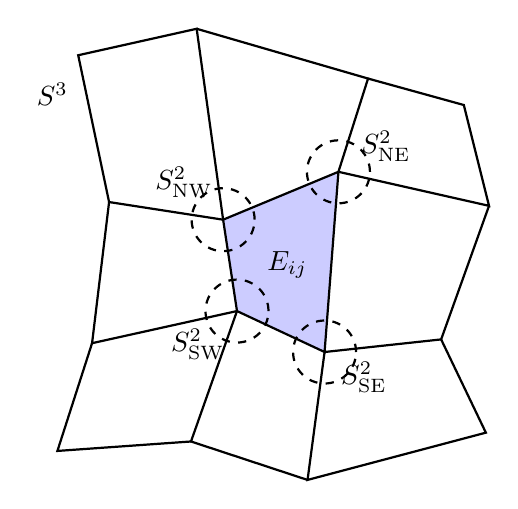
\begin{tikzpicture}[xscale=1.6, yscale = 1.6]
    \coordinate(P0) at (-0.225,0.025);
    \coordinate(P1) at (0.835,0.1);
    \coordinate(P2) at (1.76,-0.205);
    \coordinate(P3) at (3.175,0.17);
    \coordinate(P4) at (0.05,0.88);
    \coordinate(P5) at (1.2,1.135);
    \coordinate(P6) at (1.895,0.81);
    \coordinate(P7) at (2.82,0.91);
    \coordinate(P8) at (0.185,2);
    \coordinate(P9) at (1.09,1.86);
    \coordinate(P10) at (2.005,2.24);
    \coordinate(P11) at (3.2,1.97);
    \coordinate(P12) at (-0.06,3.165);
    \coordinate(P13) at (0.88,3.375);
    \coordinate(P14) at (2.24,2.98);
    \coordinate(P15) at (3,2.77);
    
    \draw [thick,-,fill=blue, fill opacity=0.2] (P5) -- (P6) -- (P10) -- (P9) -- cycle;
    \draw [thick,-] (P5) -- (P4) -- (P8) -- (P9);
    \draw [thick,-] (P9) -- (P13)-- (P12) -- (P8);
    \draw [thick,-] (P13)-- (P14)-- (P10);
    \draw [thick,-] (P14)-- (P15)-- (P11) -- (P10);
    \draw [thick,-] (P11)-- (P7)-- (P6);
    \draw [thick,-] (P6)-- (P2)-- (P3) -- (P7);
    \draw [thick,-] (P2)-- (P1) -- (P5);
    \draw [thick,-] (P1)-- (P0)-- (P4);
    
    \draw [thick, dashed] (P6) circle (.25cm);
    \draw [thick, dashed] (P5) circle (.25cm);
    \draw [thick, dashed] (P10) circle (.25cm);
    \draw [thick, dashed] (P9) circle (.25cm);
    
    \draw [thick] (1.6, 1.5) node[]{$E_{ij}$};
    
    \draw [thick] (P6) node[below, xshift = .5cm, yshift = -.0cm]{$S^2_\text{SE}$};
    \draw [thick] (P5) node[below, xshift = -.5cm, yshift = -.1cm]{$S^2_\text{SW}$};
    \draw [thick] (P9) node[above, xshift = -.5cm, yshift = .15cm]{$S^2_\text{NW}$};
    \draw [thick] (P10) node[above, xshift = .6cm, yshift = .0cm]{$S^2_\text{NE}$};
    
    \draw [thick] (P12) node[left, yshift = -.5cm]{$S^3$};
  
\end{tikzpicture}

}

\subhead{Nonlinear weights}
\begin{equation*}
    \begin{aligned}
    \hat{\alpha} &= \frac{\alpha}{(\epsilon+ \sigma_{P^3})^\tau}, \quad \hat{\beta}_k &&= \frac{\beta_k}{(\epsilon+ \sigma_{P_k^2})^\tau}\\
     \tilde{\alpha} &= \frac{\alpha}{\hat{\alpha} + \sum_{l\in I}\hat{\beta}_l}, \quad \tilde{\beta}_k &&= \frac{\beta_k}{\hat{\alpha} + \sum_{l\in I}\hat{\beta}_l}
    \end{aligned}
\end{equation*}
\Maroon{Smoothness Indicator}
\begin{equation*}
\sigma_{p^r} = \sum_{l=1}^{r-1}\int_{E_i} \Delta x_i^{2l-1}(\frac{d^l}{dx^l}P^r(x))^2 dx
\end{equation*}

\end{myslideNoFooter}

\begin{myslideNoFooter}
\heading{WENO-AO(4,3) Reconstruction}
\bigskip
\parbox{0.6\textwidth}{\raggedright
Because WENO-AO(4,3) is used in reconstruction of diffusive term. The fourth order reconstruction should 
be reconstructed in a symmetric manner to avoid directional bias.
\begin{equation*}
\begin{aligned}
 b_x(x) \approx R_i^{4,3}(x) = \frac{\tilde \alpha}{\alpha}[Q^{4'}(x) &- \sum_{k\in I}\beta_k Q_k^{3'}(x)] \\
                                                               &+ \sum_{k\in I}\tilde \beta_k Q_k^{3'}
 \end{aligned}
\end{equation*}
}\parbox{0.4\textwidth}{\setlength\unitlength{4.5pt}
\begin{tikzpicture}[xscale=1.6,yscale=1.6]
    \coordinate(P0) at (-0.225,0.025);
    \coordinate(P1) at (0.835,0.1);
    \coordinate(P2) at (1.76,-0.205);
    \coordinate(P3) at (3.175,0.17);
    \coordinate(P4) at (0.05,0.88);
    \coordinate(P5) at (1.2,1.135);
    \coordinate(P6) at (1.895,0.81);
    \coordinate(P7) at (2.82,0.91);
    \coordinate(P8) at (0.185,2);
    \coordinate(P9) at (1.09,1.86);
    \coordinate(P10) at (2.005,2.24);
    \coordinate(P11) at (3.2,1.97);
    \coordinate(P12) at (-0.06,3.165);
    \coordinate(P13) at (0.88,3.375);
    \coordinate(P14) at (2.24,2.98);
    \coordinate(P15) at (3,2.77);

    \coordinate(P16) at (0.05,-1,1);
    \coordinate(P17) at (1.01,-0.8);
    \coordinate(P18) at (1.95,-1);
    \coordinate(P19) at (3.1,-1.2);
    \coordinate(P20) at (4,-1.1);
    \coordinate(P21) at (0,4);
    \coordinate(P22) at (1.1,4.1);
    \coordinate(P23) at (2.05,4.025);
    \coordinate(P24) at (3,3.9);
    \coordinate(P25) at (4,4);

    \coordinate(P26) at (4.1,0);
    \coordinate(P27) at (3.9,1);
    \coordinate(P28) at (4.05,2);
    \coordinate(P29) at (4,3);
    
    \coordinate(C0) at (1.4,0.5);
    \coordinate(C1) at (2.5,0.5);
    \coordinate(C2) at (1.5,2.6);
    \coordinate(C3) at (2.5,2.6);

    \draw [thick,-,fill=blue, fill opacity=0.2] (P5) -- (P6) -- (P10) -- (P9) -- cycle;
    \draw [thick,-] (P5) -- (P4) -- (P8) -- (P9);
    \draw [thick,-] (P9) -- (P13)-- (P12) -- (P8);
    \draw [thick,-] (P13)-- (P14)-- (P10);
    \draw [thick,-] (P14)-- (P15)-- (P11) -- (P10);
    \draw [thick,-,fill=blue, fill opacity=0.2] (P10)--(P11)-- (P7)-- (P6) -- cycle;
    \draw [thick,-] (P6)-- (P2)-- (P3) -- (P7);
    \draw [thick,-] (P2)-- (P1) -- (P5);
    \draw [thick,-] (P1)-- (P0)-- (P4);

    \draw [thick,-] (P0)-- (P16)-- (P17)-- (P18)-- (P19)--(P20);
    \draw [thick,-] (P12)-- (P21)-- (P22)-- (P23)-- (P24)--(P25);
    \draw [thick,-] (P20)--(P26)-- (P27)-- (P28)-- (P29)--(P25);

    \draw [thick,-] (P22)-- (P13);
    \draw [thick,-] (P23)-- (P14);
    \draw [thick,-] (P24)-- (P15);
    \draw [thick,-] (P17)-- (P1);
    \draw [thick,-] (P18)-- (P2);
    \draw [thick,-] (P19)-- (P3);
    \draw [thick,-] (P26)-- (P3);
    \draw [thick,-] (P27)-- (P7);
    \draw [thick,-] (P28)-- (P11); 
    \draw [thick,-] (P29)--(P15);
   
    \draw [thick] (2,1.8) node[cross,rotate=30] {};

    \draw [thick] (2,1.8)-- (1.5,1.8);
    \filldraw[black] (1.5,1.8) circle (1.2pt) node[anchor=west] {};
    
    \draw [thick] (1.5,1.8)-- (0.6,1.8);
    \filldraw[black] (0.6,1.8) circle (1.2pt) node[anchor=west] {};
    
    \filldraw[black] (1.97,1.8) circle (1.1pt) node[anchor=west] {};
    
    \draw [thick] (2,1.8)-- (2.5,1.8);
    \filldraw[black] (2.5,1.8) circle (1.2pt) node[anchor=west] {};
    
    \draw [thick] (2.5,1.8)-- (3.6,1.8);
    \filldraw[black] (3.6,1.8) circle (1.2pt) node[anchor=west] {};
    

    \draw [thick, dashed] (C0) circle (24pt);
    \draw [thick, dashed] (C1) circle (24pt);
    \draw [thick, dashed] (C2) circle (24pt);
    \draw [thick, dashed] (C3) circle (24pt);
    
    \draw [thick] (1.6, 1.5) node[]{$E_{ij}$};
    \draw [thick] (2.6, 1.5) node[]{$E_{i+1,j}$};
    
    \draw [thick] (C0) node[below, xshift = -0.1cm, yshift = 0.2cm]{$S^3_\text{SW}$};
    \draw [thick] (C1) node[below, xshift = 0.15cm, yshift = 0.2cm]{$S^3_\text{SE}$};
    \draw [thick] (C2) node[above, xshift = -0.175cm, yshift = -0.05cm]{$S^3_\text{NW}$};
    \draw [thick] (C3) node[above, xshift = 0.2cm, yshift = -0.35cm]{$S^3_\text{NE}$};
    
    \draw [thick] (P12) node[left, yshift = -.5cm]{$S^4$};
  
\end{tikzpicture}

}

\bigskip
\bigskip
The details of WENO-AO(3,2) and WENO-AO(4,3) reconstruction can be found in reference [2].
\end{myslideNoFooter}

\begin{myslideNoFooter}
\heading{A Lax-Friedrichs Type Numerical Flux}
\subhead{Normal flux and Jacobian}
\begin{equation*}
F(U)\nu = \twoVec({\v_e\cdot\nu\,\bar c},{\v_e^E\cdot\nu\,E})
\end{equation*}
and
\begin{equation*}
    \frac{\d F(U)\nu}{\d U} = \left[\begin{matrix}
    \frac{\d(\v_e\cdot\nu\,\bar c)}{\d\bar c}
        &\frac{\d(\v_e\cdot\nu\,\bar c)}{\d E}\\[4pt]
    \frac{\d(\v_e^E\cdot\nu\,E)}{\d\bar c}
        &\frac{\d(\v_e^E\cdot\nu\,E)}{\d E}
    \end{matrix}\right]
    \approx
    \left[\begin{matrix}
    \v_e\cdot\nu&0\\
    0&\v_e^E\cdot\nu
    \end{matrix}\right].
\end{equation*}

\subhead{Lax-Friedrichs flux}\newline
Replace this normal flux with $\hat F(U^-,U^+)$, where $U^-$ and $U^+$ are one-sided limits of the approximate solution.
\begin{equation}
    \hat F(U^-,U^+)
    = \tfrac12\big[F(U^-)\nu + F(U^+)\nu
    - \Maroon{\alpha_{\textrm{LF}}}(U^+ - U^-)\big],
\end{equation}
where
\begin{equation}
    \Maroon{\alpha_{\textrm{LF}}} =  \left[\begin{matrix}
    \|\v_e\cdot\nu\|_{L^\infty}&0\\
    0&\|\v_e^E\cdot\nu\|_{L^\infty}
    \end{matrix}\right].
\end{equation}

\end{myslideNoFooter}

\begin{myslideNoFooter}
\heading{Implicit Solver}
We discretize time into levels $t^0<t^1<t^2<\cdots$ and set $\dt^{n+1} = t^{n+1}-t^{n}$. The time derivative will be integrated over the interval $[t^n,t^{n+1}]$ using a third order Runge-Kutta time stepping method.

\subhead{Radau-IIA method} A third order implicitt Runge-Kutta method. A Butcher Tableau for this mehtod is presented.\newline
\begin{center}
    \begin{tabular}{c | c c}
        1/3 & 5/12 & $-1/12$ \\
        1  & 3/4  & 1/4 \\
        \hline
          & 3/4 & 1/4
    \end{tabular}
\end{center}

\subhead{Remark.}\newline
Radau-IIA method is simple and L-stable at the same time.

\end{myslideNoFooter}

\separatorHeading{Two Different Algorithms}

\begin{myslideNoFooter}
\heading{Sequential solver}

\begin{algorithm}[H]
\caption{Sequential solution\label{alg:sequential}}
\SetAlgoLined
 Let $U^0$ be given as initial data.
 
 Initialize:
 \begin{enumerate}
     \item Given $U^0$, compute $W^0$ by the flash calculation.
     \item Given $\phi_f^0$ in $W^0$, solve the Darcy-Stokes system for $V^{0}$.
\end{enumerate}
 
 \For{\rm Time level $n=0,1,\ldots,n_{\max}-1$}{
 \begin{enumerate}
     \item Given $W^n$ and $V^n$, define
        \begin{equation*}
            \kappa^n = \frac{\phi_f^nc_f^n}{\bar c^n}
            \qquad\text{and}\qquad
            \lambda^n = \frac{\phi_f^n\rho_fe_f^n}{E^n},
        \end{equation*}
        and then solve the transport system for $U^{n+1}$.
     \item Given $U^{n+1}$, compute $W^{n+1}$ by the flash calculation.
     \item Given $\phi_f^{n+1}$ in $W^{n+1}$, solve the Darcy-Stokes system for $V^{n+1}$.
  \end{enumerate}
 }
 \end{algorithm}

\subhead{Notation.}
\begin{blist}
\item $V^n=(\v_{h,r}^n,\v_{h,s}^n,q_{h,f}^n,q_h^n)$ denote the solution to the Darcy-Stokes system at the same time.
\item $W^n=(\phi_f^n,c_f^n,T^n,\phi_1^n)$ denote the output of the flash calculation at $t^n$.
\end{blist}

\end{myslideNoFooter}

\begin{myslideNoFooter}
\heading{Iteratively Coupled solver}
\begin{algorithm}[H]
\caption{Iteratively coupled solution\label{alg:iterative}}
\SetAlgoLined
%\KwResult{Write here the result }
 Let $U^0$ be given as initial data.
 
 Initialize $W^0$ and $V^0$ as in Algorithm~\ref{alg:sequential}.
 %\begin{enumerate}
 %    \item Given $U^0$, compute $W^0$ by a flash calculation.
 %    \item Given $\phi_f^0$ in $W^0$, solve the Darcy-Stokes system for $V^{0}$.
 %\end{enumerate}
 
 \For{\rm Time level $n=0,1,\ldots,n_{\max}-1$}{
    Set $U^{n,0}=U^n$, $V^{n,0}=V^n$, and $W^{n,0}=W^n$.
    
    \For{\rm Newton iteration $\ell=0,1,\ldots$ until convergence (or $\ell_{\max}-1$)}{
    \begin{enumerate}
        \item Given $W^{n,\ell}$ and $V^{n,\ell}$, define
            \begin{equation*}
                \kappa^{n,\ell} = \frac{\phi_f^{n,\ell}c_f^{n,\ell}}{\bar c^{n,\ell}}
                \quad\text{and}\quad
                \lambda^{n,\ell} = \frac{\phi_f^{n,\ell}\rho_fe_f^{n,\ell}}{E^{n,\ell}},
            \end{equation*}
            \parbox{0.8\textwidth}{and then solve the transport system for $U^{n,\ell+1}$. Evaluate $U$ and $W$ at their proper times within the equation (i.e., at time $t^n$, or at time $t^{n+1}$ using the $(n,\ell)$ values, or by interpolating these two values to an intermediate time).}
        \item Given $U^{n,\ell+1}$, compute $W^{n,\ell+1}$ by the flash calculation.
        \item Given $\phi_f^{n,\ell+1}$ in $W^{n,\ell+1}$, solve the Darcy-Stokes system 
        for $V^{n,\ell+1}$.
    \end{enumerate}
    }
    Set $U^{n+1}=U^{n,\ell+1}$, $V^{n+1}=V^{n,\ell+1}$, and $W^{n+1}=W^{n,\ell+1}$.
 }
\end{algorithm}
\end{myslideNoFooter}

\begin{myslideNoFooter}
\heading{Discussion}
\subhead{Algorithm 1.} \newline
$U^{n+1}$ is computed using fixed in time values for the effective velocities $\v_e$ and $\v_e^E$, pre-calculated from the Darcy-Stokes part, and the partition functions $\kappa$ and $\lambda$. These quantities are only updated before commencing to the next time step.

\subhead{Algorithm 2.} \newline
Use the current information within a monolithic quasi-Newton solve. It still reduces to solving the three subproblems.  We simply omit the Newton derivative couplings between the subproblems. However, we will also explore improving the partition function approach by linearizing them, i.e., for $\kappa$,
\[
    \kappa = \kappa^{n,\ell} + d\kappa^{n,\ell} (U^{n,\ell+1} - U^{n,\ell}),
\]
and similarly for $\lambda$.  This will require computing derivatives of $\kappa$ and $\lambda$ in the flash package.

\end{myslideNoFooter}

\separatorHeading{\outno Application to Mantle Dynamics}
\begin{myslideNoFooter}
\heading{Application}
\subhead{Simulation of partial melting beneath mid-ocean ridges.}
\begin{nlist}
\item The high resolution transport scheme proposed by us will provide a
detailed simulation result of melt transport and segregation.
\bigskip
\item Lead to a better understand of the dynamics of mid-ocean ridges and hotpots by resolving the small scale dynamics of these processes in solitary waves.
\bigskip
\item The possible degeneracies in the porosity will be well represented and the survial of distinct geochemical signatures in the decompaction channel will also be invested.
\end{nlist}

\end{myslideNoFooter}

% =========================================================
\separatorHeading{\outno Some Preliminary Numerical Results}

% ===========================================================
\begin{myslideNoFooter}
\heading{Code Details}
\begin{blist}
\item Parallelization will be implemented with data management provided by PETSc.
\bigskip
\item Nonlinear solver and preconditioner will be controlled through PETSc functions.
\bigskip
\item Simple linear solver will be supplied by LAPACK.
\bigskip
\item Output will be HDF5 format with the help of CGNS (CFD General Notation System).
\end{blist}

\end{myslideNoFooter}

\begin{myslideNoFooter}
		  \heading{Visualization of Quadrilateral mesh with CGNS}
		  \bigskip
		  \subhead{Example output of quadrilateral mesh.}
		  \begin{center}
					 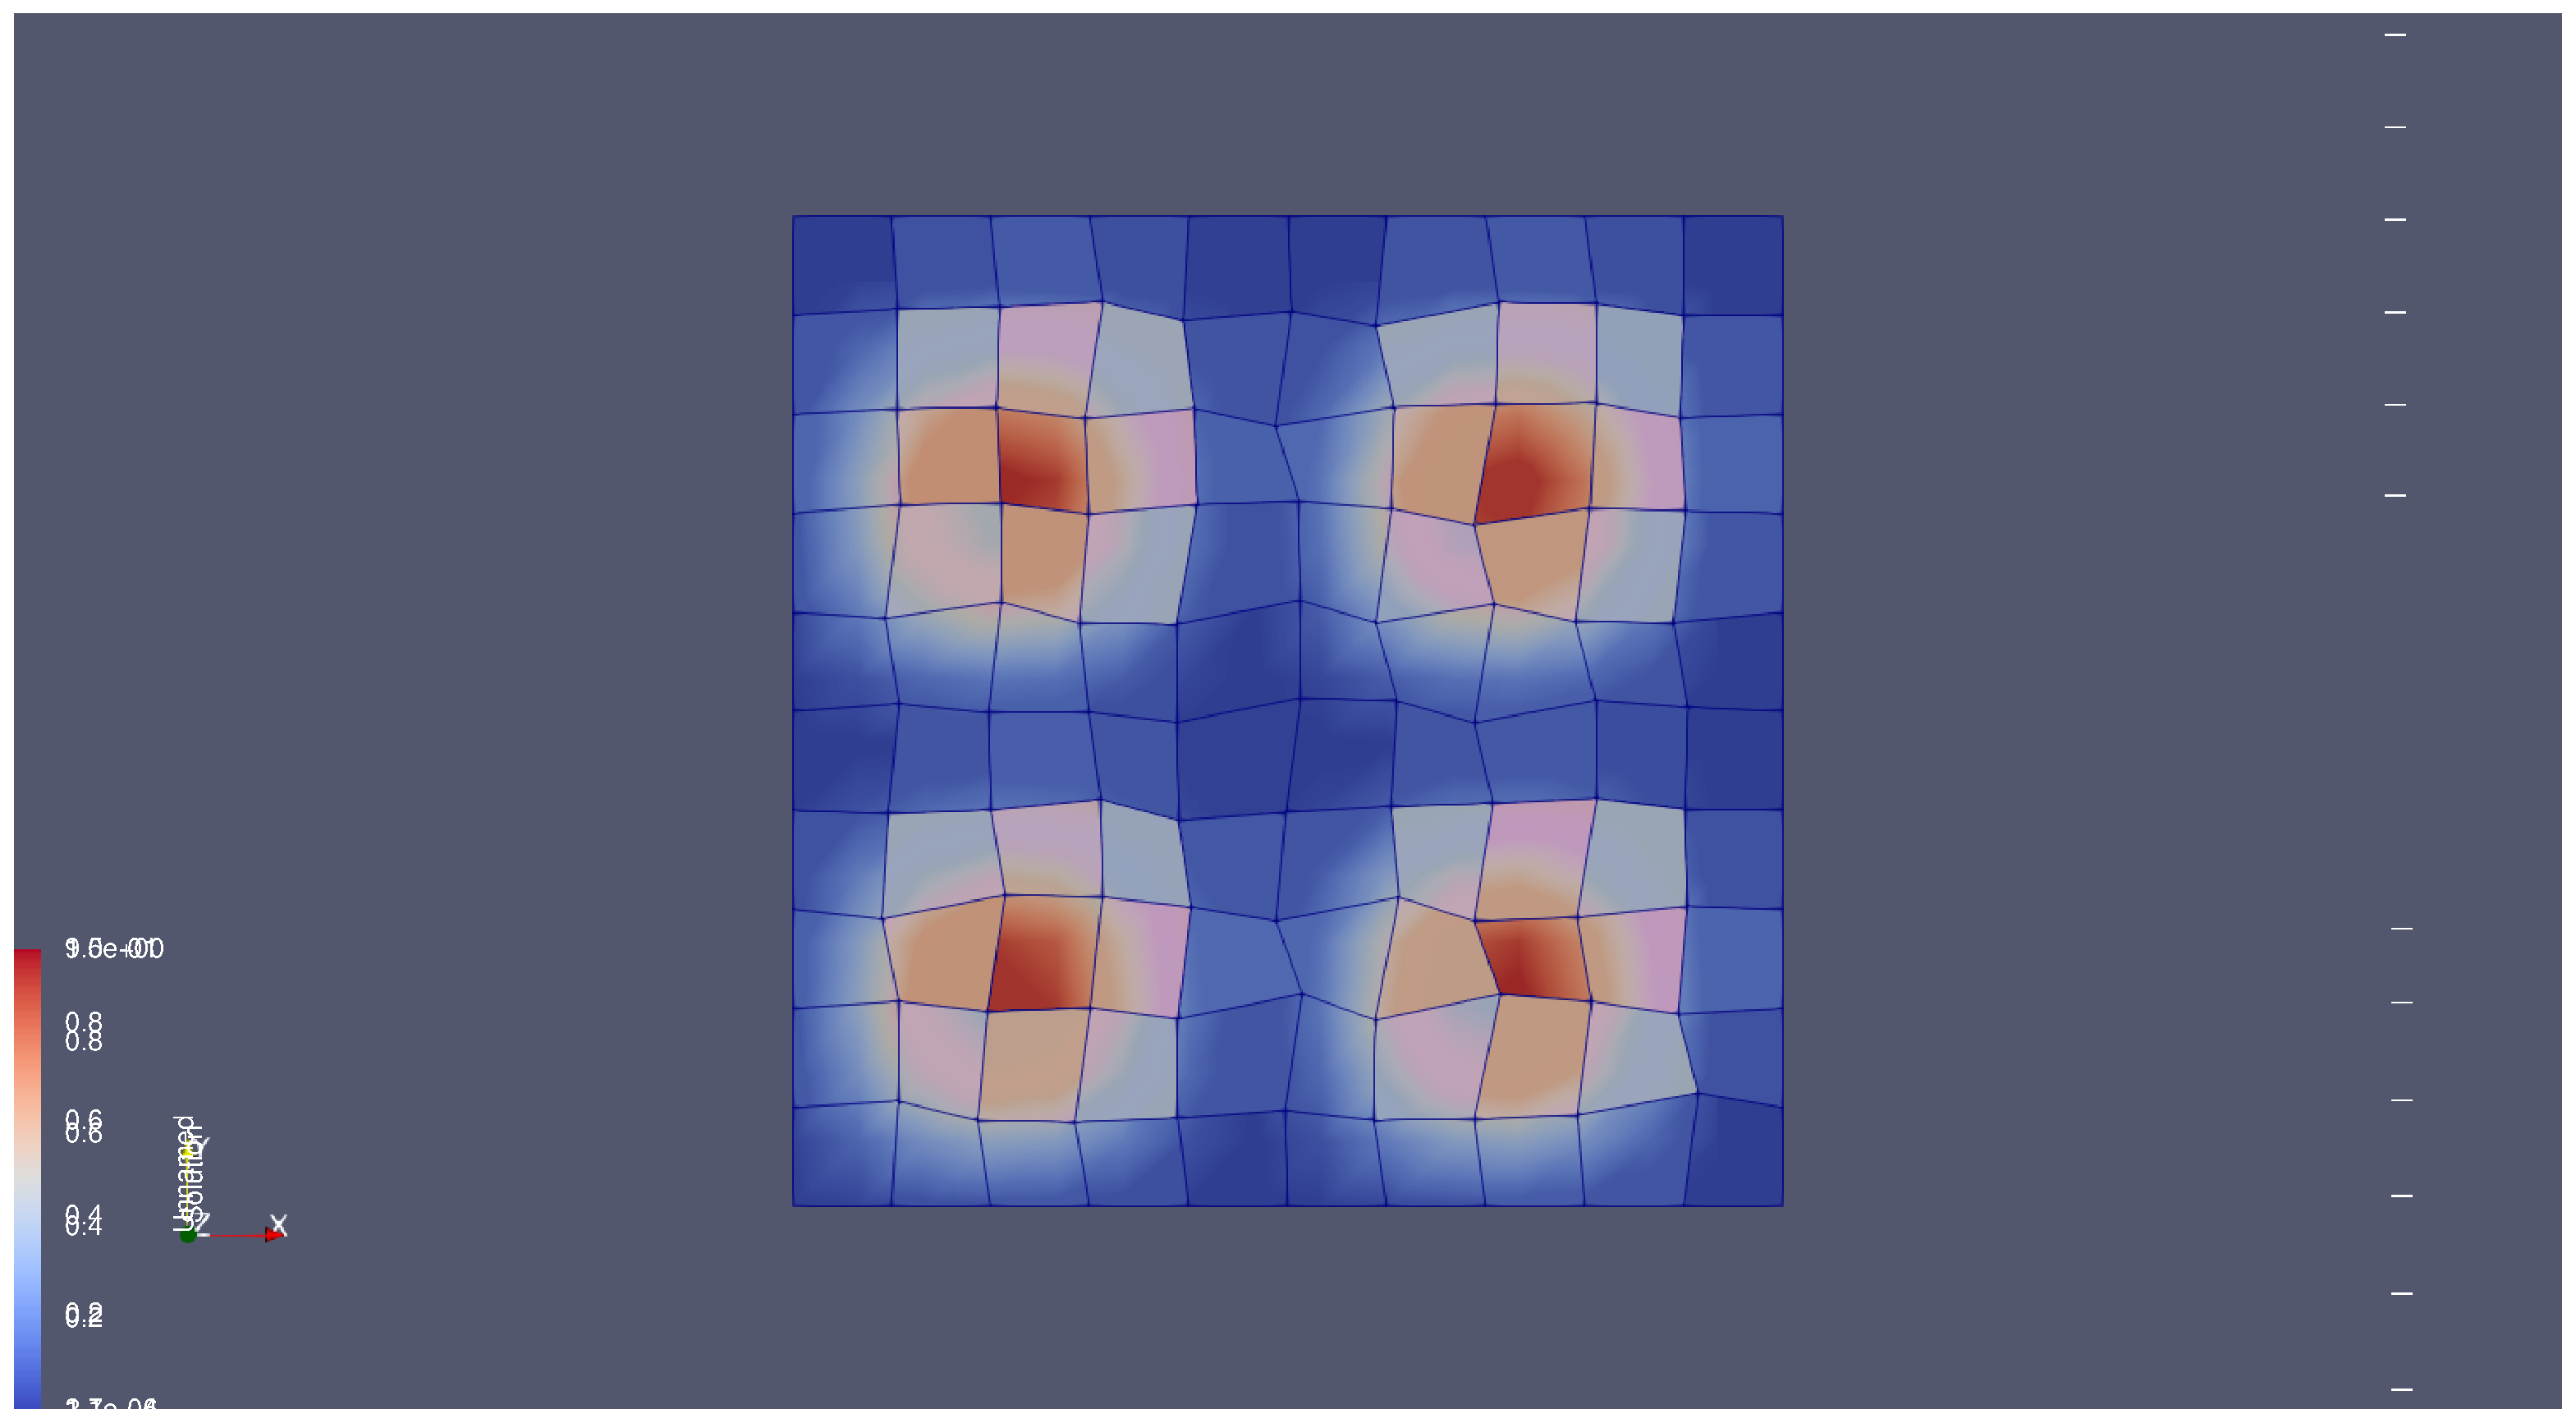
\includegraphics[width=15cm,height=10cm]{mesh.eps}
		  \end{center}
		  \subhead{Remarks.}
		  \begin{blist}
		  \item Can fit complex geometry.
		  \item Require fewer elements than triangular mesh.
		  \item Require mesh quality check.
		  \item Constructed by randomly distortion.
		  \end{blist}
\end{myslideNoFooter}
% ==========================================================
\begin{myslideNoFooter}
		  \heading{1D implicit WENO3 solver}
		  A simple 1D Burgers equation with periodic boundary condition has been solved with the
PETSc-based code. The implicit WENO3 method was used
here. 
\begin{equation*}
u_t + \frac{u^2}{2} = 0
\end{equation*}

\subhead{Computed numerical result}
		  \begin{center}
					 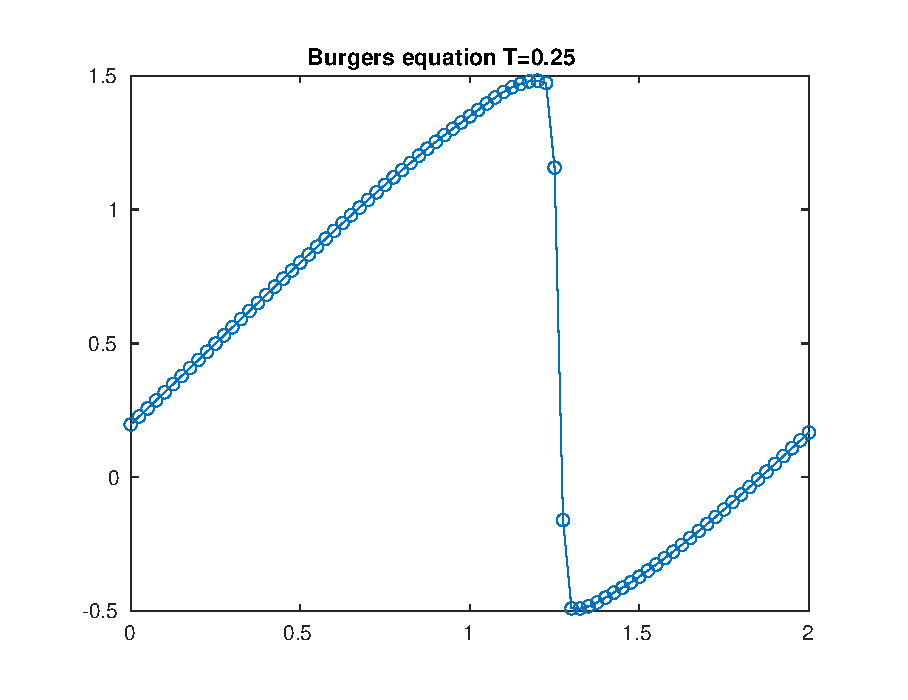
\includegraphics[width=12cm,height=10cm]{1d.eps}
		  \end{center}
\end{myslideNoFooter}
% ===========================================================
\begin{myslideNoFooter}
		  \heading{Convergence Test for New BR Element}
           \subhead{Analytical result}
\begin{alignat*}2
&u = \cos(x)\sin(y), \quad && v= -\sin(x)\cos(y), \\
&\frac{\partial p}{\partial x} = \cos(x)\sin(y), \quad && \frac{\partial p}{\partial y}= \sin(x)\cos(y).
\end{alignat*}

\subhead{Computed numerical result}
        \begin{center}
					 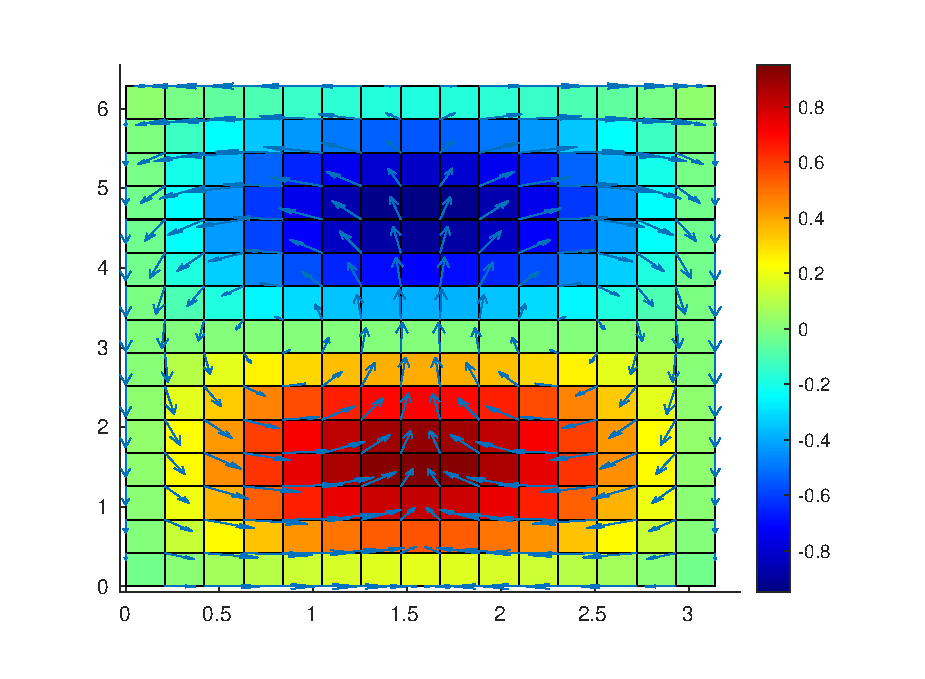
\includegraphics[width=8cm,height=7cm]{ex2.eps}
					 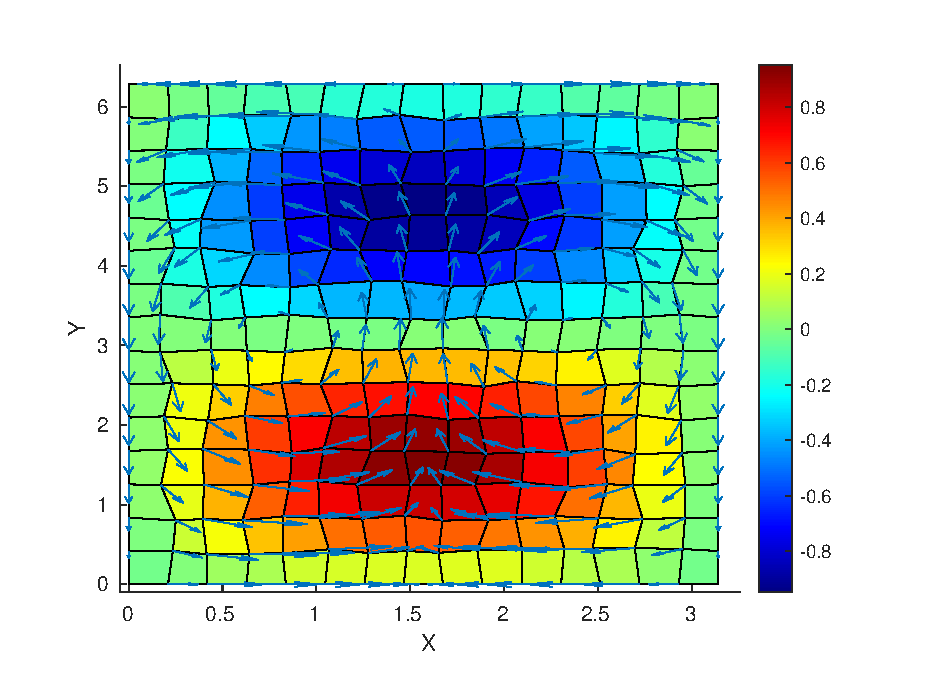
\includegraphics[width=8cm,height=7cm]{ex1.eps}
		  \end{center}
The computed numerical result is compared to this exact solution by calculating the $L^2$ norm of the residual (i.e., the difference) of the pressure, velocity, and derivative of velocity.

\end{myslideNoFooter}

\begin{myslideNoFooter}
\subhead{Rectangular mesh}
\bigskip
\begin{center}
     \begin{tabular}{c | c c c c}
     Grid size & $8\times8$ & $16\times 16$ & $32\times32$ & $64 \times 64$ \\
     \hline
     $L^2(\text{res}_u)$ & 4.502E$-$1 & 1.052E$-$1 & 2.513E$-$2 & 6.130E$-$3 \\
     $L^2(\text{res}_p)$ & 1.039E+0 & 4.463E$-$1 & 2.093E$-$1 & 1.019E$-$1 \\
     $L^2(\text{res}_{du})$ & 2.632E$+$0 & 5.845E$-$1 & 1.374E$-$1 & 3.330E$-$2 \\
    \end{tabular} 
    \end{center}
\subhead{Quadrilateral mesh}
\bigskip
\begin{center}
    \begin{tabular}{c | c c c c}
     Grid size & $8\times8$ & $16\times 16$ & $32\times32$ & $64 \times 64$ \\
     \hline
     $L^2(\text{res}_u)$ & 4.603E$-$1 & 1.074E$-$1 & 2.567E$-$2 & 6.266E$-$3 \\
     $L^2(\text{res}_p)$ & 1.070E$+$0 & 4.670E$-$1 & 2.207E$-$1 & 1.078E$-$1 \\
     $L^2(\text{res}_{du})$ & 2.685E$+$0 & 5.981E$-$1 & 1.525E$-$1 & 4.580E$-$2 \\
    \end{tabular}
\end{center}

\bigskip
\subhead{Remark.}
\begin{blist}
\item The order of accuracy does not degenerate on quadrilateral mesh as expected.
\item Second order accuracy for velocity and pressure. 
\item First order accuracy for derivatives of the velocity.
\end{blist}
\end{myslideNoFooter}

\separatorHeading{\outno Summary}

\begin{myslideNoFooter}
\begin{blist}
\item \Blue{Area A:}
\begin{nlist}
\item A new and simpler local mass conservative mixed finite element scheme for the Darcy-Stokes system.
\item A modified Bernardi-Raugel element equiped with direct serendipity space. The stability and convergence
of this new element will be further studied.
\item Analyze propagation of errors within the discrete coupled system.
\item Analyze mass conservation in the context of the complete coupled system of equations.
\end{nlist}
\item \Blue{Area B:}
\begin{nlist}
\item A PETSc implementation of the proposed algorithm. Parallel running will be enabled in the solver.
\item The suitability of the linearized formulation of $\kappa$  and $\lambda$ will be studied.
\item The suitability of Lax-Friedrichs type numerical flux.
\item First implement of the implicity WENO-AO method in full scale mantle simulation.
\end{nlist}
\end{blist}
\end{myslideNoFooter}

\begin{myslideNoFooter}
\begin{blist}
\item Area C
\begin{nlist}
\item New partition function method will be compared with standard approach proposed by Katz.
\item New local mass conservation scheme will be studied from a physical point of view.
\item Expect to see a improved approximation of the dynamics of partial melting in simulatins of 
melt extraction beneath mid-ocean ridge.
\end{nlist}
\end{blist}
\end{myslideNoFooter}

\separatorHeading{ Future Work and Timeline}

\begin{myslideNoFooter}
\heading{Future Work}
\begin{nlist}
\item Continue studying new mixed finite element space.
\bigskip
\item \Maroon{Develop a feasible code}.
\bigskip
\item Perform numerical simulation of real world problems.
\end{nlist}
\end{myslideNoFooter}

\begin{myslideNoFooter}

\heading{Timeline Gantt Chart}

\begin{center}
\begin{ganttchart}[vgrid,hgrid,bar/.append style={fill=black!50},inline,
today = 3,x unit=0.73cm,
y unit title=2cm,
y unit chart=1.6cm,
group label font=\tiny\bfseries,
milestone label font=\tiny\itshape,
bar label font=\tiny,
title label font=\tiny]{1}{36}
%labels
\gantttitle{Semesters}{36}\\
\gantttitle{20 Fall}{4}
\gantttitle{21 Spring}{5}
\gantttitle{21 Sum}{3}
\gantttitle{21 Fall}{4}
\gantttitle{22 Spring}{5}
\gantttitle{22 Sum}{3}
\gantttitle{22 Fall}{4}
\gantttitle{23 Spring}{5}
\gantttitle{23 Sum}{3}\\

%\ganttgroup{Area A}{1}{30}\\
\ganttbar{New BR Element}{1}{10}\\
\ganttbar{Partition Function}{8}{15}\\
\ganttbar{Error Analysis}{8}{20}\\
\ganttbar{Algorithm Analysis}{12}{22}\\
%\ganttgroup{Area B}{1}{30}\\
\ganttbar{Code Development}{1}{22}\\
\ganttlinkedbar{Mantle Simulation}{23}{32}\\
\ganttbar{Code Optimization}{23}{32}\\
\ganttbar{Dissertation}{26}{36}
%\ganttgroup{Area C}{1}{30}

\end{ganttchart}
\end{center}

\end{myslideNoFooter}

\begin{myslideNoFooter}
\heading{Reference}
\begin{nlist}
\item T. Arbogast and A. L. Taicher, \Blue{\em A linear degenerate elliptic equation arising from
    two-phase mixtures,} SIAM J.\ Numer.\ Anal. 54:5 (2016), pp. 3105-3122. DOI 10.1137/16M1067846.
\item T. Arbogast, C.-S. Huang, and X. Zhao, \Blue{\em Accuracy of WENO and adaptive order WENO reconstructions for solving conservation laws}, SIAM. J.\ Numer.\ Anal., 56 (2018), pp. 1818–1847. DOI 10.1137/17M1154758.
\item T. Arbogast, M. A. Hesse, and A. L. Taicher, \Blue{\em Mixed methods for two-phase
    Darcy-Stokes mixtures of partially melted materials with regions of zero porosity,} SIAM J.\
  Sci.\ Comput.\ 39:2 (2017), pp.~B375--B402. DOI 10.1137/16M1091095.

\end{nlist}
\end{myslideNoFooter}

% add timeline

% add summary

% about 45 slides


\end{document}
